\documentclass[a4paper]{report} % paper size and format

\usepackage{titling} % to use \thetitle, \theauthor, etc.
\title{Oil Temperature Control Unit}
\author{Ediz Ferit Kula \and Serdal Şen}
\date{January 2023}

% load packages:
\usepackage[margin=1in]{geometry}   % edit page margins
\usepackage{indentfirst}            % indent after section title
\setlength\parindent{24pt}
\usepackage{setspace}               % line spacing
\setstretch{1.25}
\usepackage{wrapfig}
\usepackage[T1]{fontenc}
\usepackage{pdfpages} % Include pdf pages as figures
\usepackage{tocloft} % Dot fill for TOC
\usepackage{siunitx} % Better units and numbers. Using v2 in this document
\usepackage[americaninductors]{circuitikz} % For drawing the schematic
\usepackage{amsmath} % Better math presentation
\usepackage{physics} % Better math presentation
\usepackage{graphicx} % Insert images
\usepackage[section]{placeins} % Force figures to appear in the section in which they are declared.
\usepackage[inkscapepath=output/.svg]{svg} % Insert svg images
\usepackage{caption} % Better caption and linking behaviour.
\usepackage{subcaption} % For subfigures
\usepackage{float} % For H float setting

%% MATLAB ==============================
\usepackage{lmodern}
\usepackage{hyperref}
\usepackage{amsmath}
\usepackage{amsfonts}
\usepackage{epstopdf}
\usepackage{matlab}
\sloppy
\epstopdfsetup{outdir=./}
\graphicspath{ {./matlab_images/} }
%% =====================================

% --------------------------------------------------------------------
% Renew commands
% --------------------------------------------------------------------
\setlength{\parskip}{10pt} % Increasing the space between paragraphs

% --------------------------------------------------------------------
% New Commands and Definitions
% --------------------------------------------------------------------

% Force figures to appear in the subsection in which they are declared:

\makeatletter
\AtBeginDocument{%
    \expandafter\renewcommand\expandafter\subsection\expandafter{%
        \expandafter\@fb@secFB\subsection
    }%
}
\makeatother




\begin{document}

    \pagenumbering{roman}

    \begin{titlepage}
        \begin{center}
            \vspace*{1cm}

    
            \LARGE
            \thetitle
            
            \Large
            \vspace{0.5cm}
            
            by
            
            \vspace{0.5cm}
            \theauthor
            
            \vfill
            
            \vspace{0.8cm}
            \includesvg[width=0.4\textwidth]{images/logo.svg}
            
            \Large
            Department of Mechanical Engineering\\
            Bogazici University\\
            Turkey\\
            \thedate
            \vspace*{1cm}
        \end{center}
    \end{titlepage}

    \begin{abstract}
         This report aims to introduce a dynamic model with Matlab/Simulink that simulates the oil cycle part of an ORC setup and proposes a solution for the oil's oscillating temperature. The heater of this cycle regularly overshoots and undershoots the set temperature of the oil, and this results in an oscillation of the temperature of the primary working fluid, which is not desired. A dynamic model is created by applying thermodynamic and heat transfer principles to the components of the oil cycle. The unknown variables are either calculated by the experimental data or found by using the experimental data as training data to the model. Afterward, the model is, compared with the experimental data to demonstrate that the model is valid; as it turned out, the model data and experimental data are coherent. Next, a proposed solution is created including a bypass pipeline between the inlet and exit and producing a reverse flow. The simulation of the proposed solution is done with the validated model. The simulation demonstrated that the oscillations could be reduced with the bypass pipeline based on how much of the flow goes through the bypass pipeline. Furthermore, a concept experimental setup is created by using a pump, a check valve, a 3-way valve, and an actuator. The real experiment, however, only consisted of a 3-way valve and an actuator, demonstrating that the 3-way valve can be controlled with the actuator to change the fluid flow direction.
    \end{abstract}
   

    \tableofcontents
    \setcounter{page}{3}
    \clearpage
    \listoffigures
    \clearpage
    \listoftables
    \clearpage

    \pagenumbering{arabic}

    \chapter{Introduction}

There is an organic rankine cycle (ORC) experiment setup located in the BURET (Bogazici University Renewable Energy Technologies) in Kilyos, Istanbul (See Figure \ref{exsetup}). The ORC setup's primary objective is to extract energy from low-temperature heat sources such as solar, waste, or biomass by using fluids with low boiling temperatures. The setup consists of two separate fluid cycles: the main working fluid cycle and the oil cycle. The oil cycle extracts energy from a heater and transfers the energy to the main working fluid. Meanwhile, hot and pressurized main working fluid spends its energy rotating a shaft that generates electricity.

\begin{figure}[H]
		\centering
		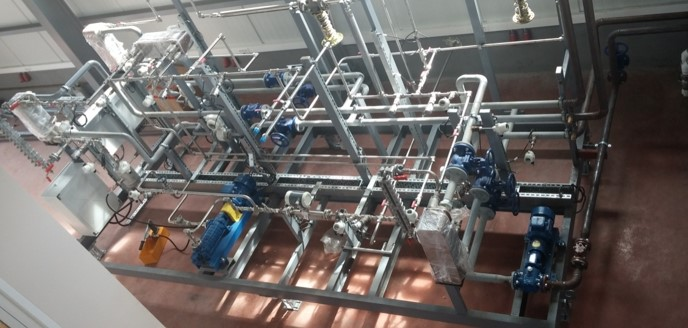
\includegraphics[width=0.6\textwidth]{images/exsetup.jpg}
		\caption[ORC Setup in BURET Lab]{ORC Setup in BURET Lab}
		\label{exsetup} 
\end{figure} 
	
The main working fluid cycle had already been investigated by Altun et al. Altun developed a dynamic simulation model that predicts the temperatures and pressures across the cycle, including the pressure and heat losses, by using Modelica and validated his model with the experiment results of the ORC setup. In this project, we focus on the other side of the ORC, the oil cycle, and we propose a way to improve the cycle.
	
The oil cycle (See Figure \ref{cycle}) consists of 4 main components: the heater, the pump, the evaporator, and the oil tank. Basically, the oil is heated at the heater, which has a resistor and an on-off temperature control unit. The hot oil is pumped toward the evaporator by a gear pump, and the oil transfers its energy to the cold main working fluid inside the evaporator, which is a plate-type heat exchanger. The heater can be controlled by setting a temperature. When the thermocouple at the exit of the heater determines a higher temperature than the set temperature, the heater is closed. When the temperature at the exit of the heater is determined to be less than the set temperature, the heater is turned on.
	
	\begin{figure}[H]
		\centering
		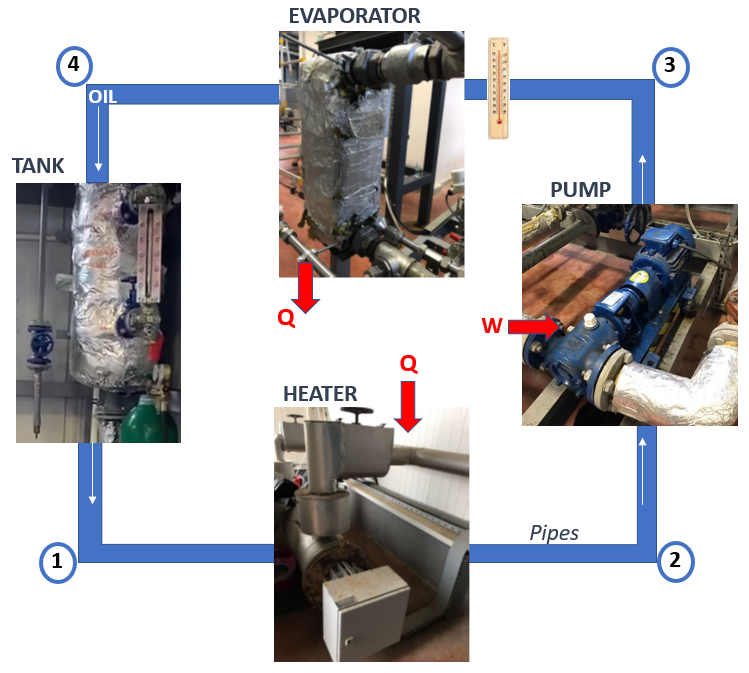
\includegraphics[width=0.56\textwidth]{images/cycle.png}
		\caption[The Oil Cycle]{The Oil Cycle}
		\label{cycle} 
	\end{figure} 
	
The problem that is aimed to be fixed in this project occurs because of the oil heater's on-off type temperature controller. The thermocouple used to determine the exit temperature at the exit has a hysteresis of $\pm 3^\circ C$. That is why the oil is either heated or left to be cooled much more than the desired set temperature. Additionally, the resistor inside the heater, which has a heating capacity of 100 kW, remains hot even after the heater is closed, resulting in an additional temperature rise after the set temperature is reached. Both of these reasons result in the oscillation of the oil temperature at the heater exit (See Figure \ref{osc}). The oscillation temperature of the oil causes the temperature of the main working fluid to oscillate.

\begin{figure}[H]
		\centering
		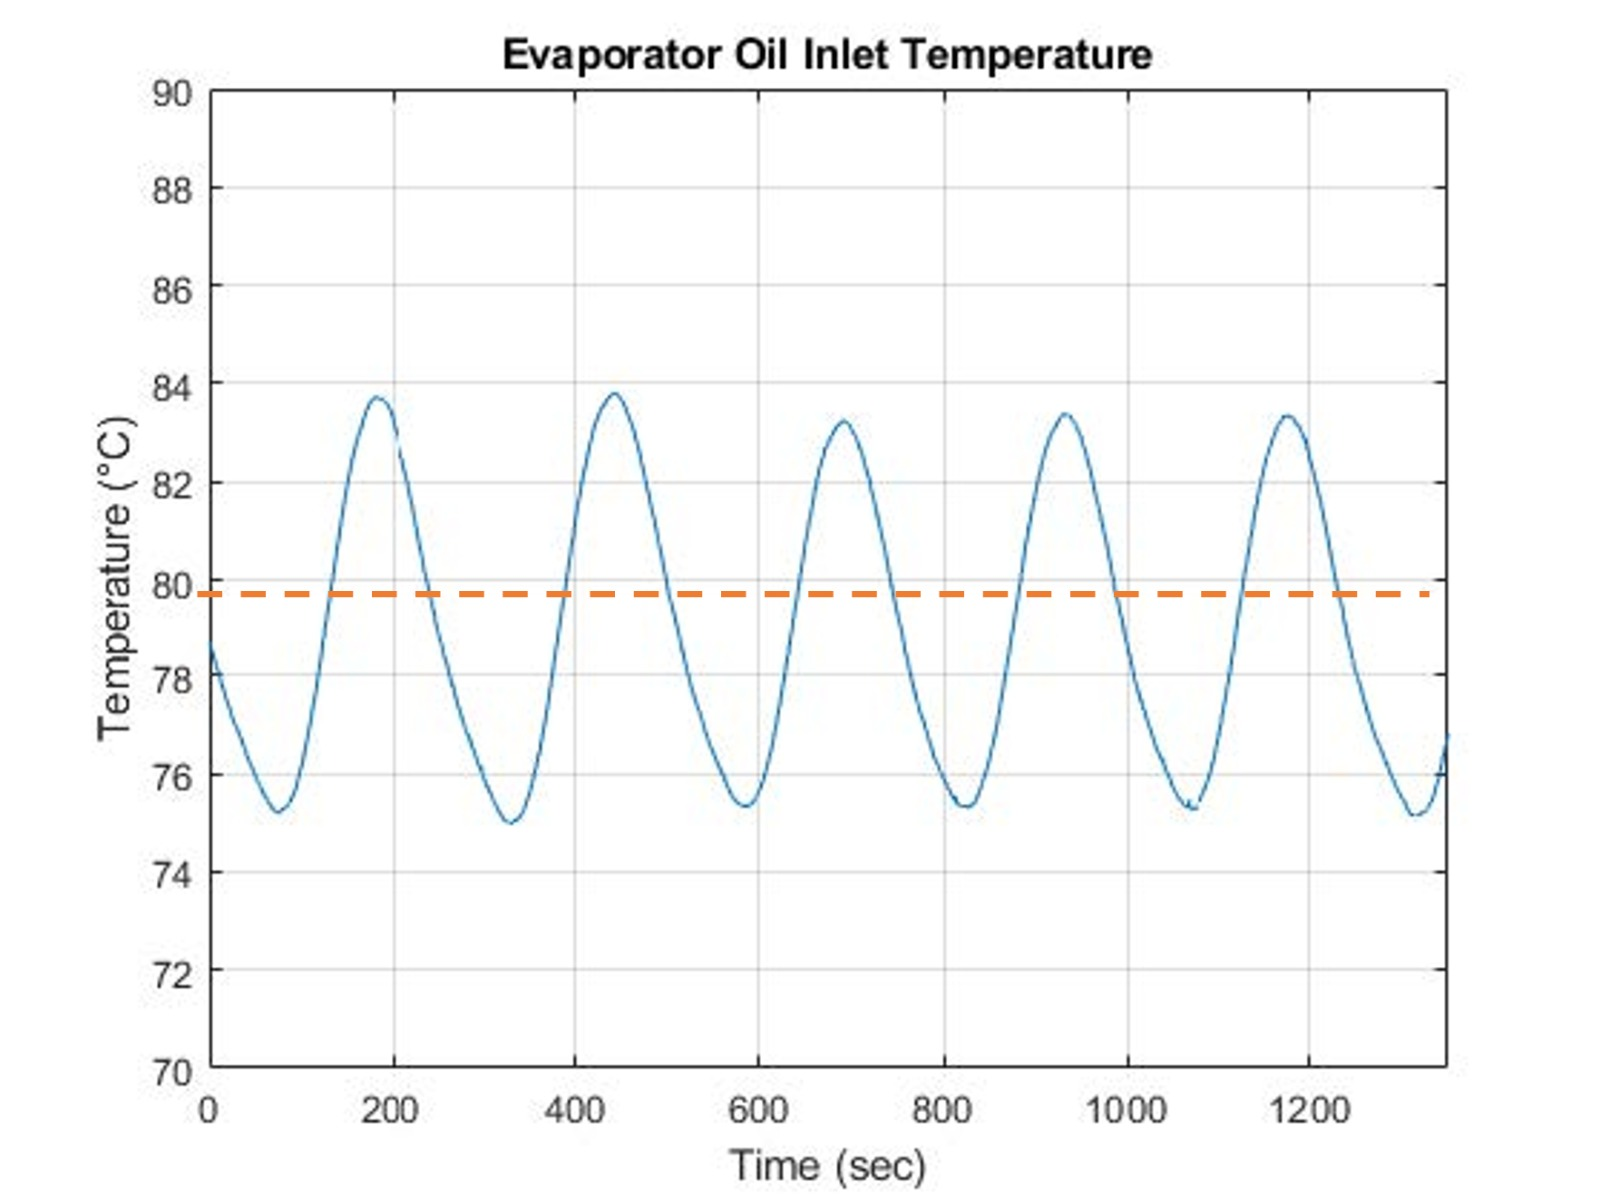
\includegraphics[width=0.6\textwidth]{images/oscillation.jpg}
		\caption[The oscillation of oil's temperature when set temperature is $80^\circ C$] {The Oscillation of Oil's temperature when set Temperature is $80^\circ C$}
		\label{osc} 
\end{figure} 

This project aims to develop a simulation model that predicts temperature across the oil cycle, propose a mechanical solution to decrease the oil oscillation, and modeling of the proposed solution. According to the literature, there is a couple of software that can be used to model a thermodynamic cycle, like ORC setups such as GtSuite, Modelica, and Matlab/Simulink.
	
An example study on the dynamic modeling of ORC and optimization of some components, such as turbines and heat exchangers, was conducted by Marchionni et al. \cite{marchi}. A 1D computer-aided modeling software called GTSuite was employed in his model. Rather than MW scale ORC systems, this research concentrates on kW scale systems. The goal of this study is to model ORC systems with power output ranging from 34.5 kW to 55.5 kW. To observe the cycle's transient reaction, various mass flow rates and intake temperatures of cooling water and hot oil are investigated.
	
Another software that can be employed to make a dynamic model for ORC is Modelica which is used by Wei et al. \cite{wei}. The cycle's heat source is a power plant's exhaust gas, and the air is used for cooling. They examined the accuracy, complexity, and simulation durations of moving boundary (MB) and finite volume (FV) methods. Results of the transient analysis are presented for both scenarios and contrasted with experimental data. It is discovered that the MB strategy is quicker and simpler than the FV approach as a result. The FV method, however, is more precise than the MB one. As a result, MB is more appropriate than the FV technique if the simulation time is the primary concern, whereas the FV approach would make more sense if it is not. Additional to Wei et al.'s study, Modelica/Dymola was used by Zhang et al. \cite{zhang}. to develop a dynamic model for kW scale ORC. Their steps were to model the components of ORC first and then compare the model's simulation results with the experiment results. As it turned out, the model's result was compatible with the results of the experiments. By validating the model, they also validated the thermal efficiency that they calculated by this model, which was 6.94\%. Other users of Modelica/Dynamo for ORC modeling were Quolin et al. \cite{quoilin}. They also compared the model results with the experiment results, and they discovered that the model was accurate. Ertugrul's research can be considered the predecessor of this project \cite{altun}. In his thesis, which is about dynamic modeling of the ORC setup (except the oil cycle section), he made a transient simulation of ORC and found out the temperature of the R134a across the ORC cycle by using Modelica/Dymola. He also considered simulating pressure losses across ORC and validated the results with the readings from the pressure sensor in ORC. Unlike his study, we neglected the pressure effects on the system since their effects are small, and it would be costly to implement pressure sensors in the oil cycle for validation.
	
Matlab/Simulink is another applicable software for the dynamic modeling of ORC. Carraro et al. \cite{carr}. made a study targeting to model and design of a small ORC setup with the help of Matlab. They investigated the ORC system's response to the oscillating temperature of the oil between 410 K and 435 K. When they compared their dynamic model's results with the experiment's results; they calculated the maximum relative error of 6.6\%.

A similar problem is solved by Akmal et al. \cite{inproceedings}. They used Matlab/Simulink to dynamically model an underfloor heating system that has an on-off type resistor. Their aim was to create a valid model that could optimize the heating of a room with underfloor heating. Similar to the heater in the oil cycle, the heater of the underfloor heating system overshoots or undershoots the set temperature because of the delayed response of the resistor.
	
As can be seen, there are many ways to create a dynamic model of a part of the ORC setup. Modelica/Dymola, GT-Suite, and Matlab/Simulink are generally used for this purpose, and they give compatible results with the results of the experiment. In this project, Matlab/Simulink is chosen to model the oil cycle. This is mainly because of time scarcity since Matlab/Simulink is a more familiar software for us, and it would take time to learn new software. Additionally, Simulink's easy-to-use and practical interface is beneficial for us.
    \chapter{Theory}

In order to provide a transient simulation model of this oil cycle, some governing equations must be established for each component in the cycle. Additionally, in order to appropriately simulate the cooling of the system when the heater is closed, the oil in the pipes must also be included in the model. Each component in the cycle (pump, tank, heater, and evaporator) can be considered as control volume, and this will allow us to write transient energy and mass balance equations inside the components. First, let's start with the mass balance equations\cite{moran}:

	\begin{equation}
		\label{mass_balance}
		\frac{d m_cv}{dt} = \dot{m}_i - \dot{m}_e 
	\end{equation}
	\noindent
	where $\dot{m}$ is the overall mass change rate inside the control volume, and $\dot{m}_i$, and $\dot{m}_e$ represent the mass transfers at the inlet and exit of the control volume, respectively.
	
	By using Equation \ref{massvol}, the mass balance equation can be modified as volumetric flow rate balance. This formulation is more useful than the mass balance equation because the volumetric flow rate is constant across the cycle.
 
	\begin{equation}
		\label{massvol}
		\dot{m} = \dot{V} \rho
	\end{equation}
	\begin{equation}
		\label{massvol2}
		\frac{d (V_{cv} \rho)}{dt}= \dot{V}_i \dot{\rho}_i - \dot{V}_e \dot{\rho}_e
	\end{equation}
	\noindent
	where $\dot{V}$ is the volumetric flow rate, and $\dot{\rho}$ is the density.
	
	Furthermore, the transient energy balance equation can be written in the control volumes (See Equation \ref{energy}).
 
	\begin{equation}
		\label{energy}
		\frac{d E_{cv}}{dt}= \dot{Q} -  \dot{W}_{cv} +\dot{m}_i(h_i + \frac{v_i^2}{2} + gz_i) - \dot{m}_e(h_e + \frac{v_e^2}{2} + gz_e)
	\end{equation}

	\noindent
	where $ E_{cv}$ is the energy inside the control volume, and with the derivative, the left side of the equation corresponds to the energy change in the control volume. The $\dot{Q}$ is the heat transferred to the control volume, $\dot{W}_{cv}$ is the work done by the control volume, $\dot{m}$ is the mass flow rate, the $h$ is the enthalpy, $v$ is the velocity of the fluid, $gz$ is the product of the gravitational acceleration and the relative height, and the subscripts $i$ and $e$ indicate the fluid at the inlet and exit, respectively. Together $\dot{m}(h+ \frac{v^2}{2} + gz)$ means energy that enters or exits the control volume with the fluid flow at the inlet or exit. The kinetic and potential effects in this equation are negligibly small, so the equation can be reduced to Equation \ref{energy2}.
 
	\begin{equation}
		\label{energy2}
		\frac{d E_{cv}}{dt}= \dot{Q} -  \dot{W}_{cv} +\dot{m}_i h_i - \dot{m}_e h_e
	\end{equation}
	
	Another important governing equation is the heat transfer equation, as can be seen in Equation \ref{heattransfer}. This equation can be used to calculate the temperature change when heat is stored inside the material. That is why $E_{st}$ indicating energy stored in the material is used instead of $Q$.
 
	\begin{equation}
		\label{heattransfer}
		E_{st}= m c (T_2 - T_1)
	\end{equation}
	\noindent
	where $m$ is the mass of the material, $c$ is the specific heat of the material, and $T_1$ and $T_2$ are the initial and final temperatures of the material, respectively. This equation can be used to calculate the temperature change of a material by knowing the energy stored in the material. However, this equation is not transient. That is why this equation must be differentiated with respect to time. Note that $T_2$ transformed to $T$ because the final temperature is unknown and desired to be calculated.
 
	\begin{equation}
		\label{heattransfer2}
		\dot{E_{st}}= \frac{d[m c (T_2 - T_1)]}{dt}
	\end{equation}
	\begin{equation}
		\label{heattransfer3}
		\dot{E_{st}}= \dot{m} c (T - T_1) + m c \frac{dT}{dt}
	\end{equation}

	The heat transfer equation and energy balance equations are related in a way. The energy balance inside a control volume determines the energy change in the control volume, which is, in our case, stored inside the oil. This relation can be shown by Equation \ref{ultimate}. Afterward, the equation can be transformed to:
 
	\begin{equation}
		\label{ultimate}
		\dot{E_{st}}= \dot{E_{cv}}
	\end{equation}
	\begin{equation}
		\label{ultimate2}
		\dot{m} c (T - T_1) + m c \frac{dT}{dt} = \dot{Q} -  \dot{W}_{cv} +\dot{m}_i h_i - \dot{m}_e h_e
	\end{equation}
	\noindent
	Here the mass flow rate is assumed as constant for the sake of simplicity. By using Equation \ref{mass_balance}, we can rewrite the $\dot{m}$ and solve for $\frac{dT}{dt}$.
 
	\begin{equation}
		\label{ultimate3}
		m c \frac{dT}{dt} = \dot{Q} -  \dot{W}_{cv} + \dot{m} (h_i - h_e) - \dot{m} c (T - T_1)
	\end{equation}

	To further improve the question, we need to introduce a specific heat-enthalpy relationship into consideration. The specific heat changes with temperature, but we can assume it is a constant since the specific heat does not change much within our temperature range. Therefore, the specific heat-enthalpy relation can be written as:
 
	\begin{equation}
		\label{specific}
		c_p (T_2 -T_1) = h_2 - h_1
	\end{equation}
	\noindent
	Implementing above equation into Equation \ref{ultimate3} results in:
 
	\begin{equation}
		\label{ultimate4}
		m c \frac{dT}{dt} = \dot{Q} -  \dot{W}_{cv} + \dot{m} c (T_1 - T) - \dot{m} c (T - T_1)
	\end{equation}
	\noindent
	The above equation can be simplified further. Note that there is no work done in any of the oil cycle's components except in the pump, which is neglected because it does a negligible effect on the oil's temperature.
 
	\begin{equation}
		\label{ultimate5}
		\frac{dT}{dt} = \frac{\dot{Q}}{mc}+ 2\frac{\dot{m}}{m}(T_1 - T) 
	\end{equation}
	
	Overall, the mass balance equation, control volume energy balance equation, and stored energy equations can be used as governing equations to create a model that can determine temperature change based on initial conditions.

    \chapter{Methodology}

\par
In order to test the proposed solution, a digital twin of the oil cycle is created with a process composed of three parts. Matlab/Simulink software is selected to model the system. For modeling, mathematical equations\cite{gasomi} and experimental results are used. The experiment was done in 2022 by Ertugrul Altun for his thesis given in \cite{altun}. 
\par
First, the governing equations, which are derived in the previous chapter, are used to create a Simulink model. All variables are determined, and missing values are calculated from experimental data by curve fitting. Secondly, free variables are fitted to the experimental data with a manual training process. Finally, the model is validated by experimental data that is reserved only for validation.
\par
Free variables:
\begin{itemize}
    \item $UA$
    \item $m_{r}c_{r}$
    \item $Q_{loss}$
\end{itemize}

\section{Modeling}

The system is composed of four main components:

\begin{enumerate}
    \item Heater 
    \item Pump
    \item Evaporator
    \item Tank
\end{enumerate}

\par
Each component has a governing differential equation that needs to be solved to give the current temperature. Therefore three differential equations are defined in three subsystems with Simulink blocks for each component. The differential equation for the pump is not defined since the pump has no effect on the oil properties. It only enables the continuity of the flow. 

\par
The volumetric flow rate is taken as constant through the entire system and for all temperatures because it barely changes through desired temperature change and for each component if the outliers are neglected. This can be seen in Figure \ref{fig:volumetric}.

\begin{figure}[h]
    \centering
    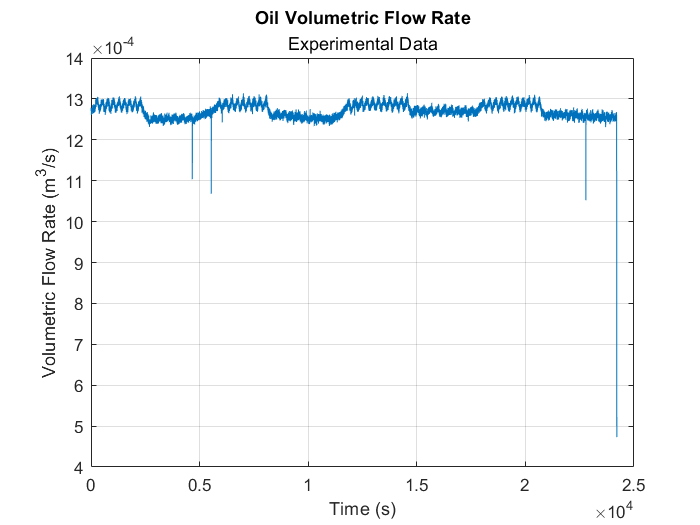
\includegraphics[width=10cm]{images/flowrate.png}
    \caption{Oil's volumetric flow rate during the experiment.}
    \label{fig:volumetric}
\end{figure}

\par
Volumetric flow rate is equal to $v = 0.001278 m^3/s$.

\par
Below assumptions are made to solve the system:
\begin{itemize}
    \item For all components, the temperature inside the component is assumed to be equal to the temperature at the exit of that component.
    \item Total heat loss in the system is assumed to be lost at the tank.
\end{itemize}

\subsection{Heater}
The heater is the place where the oil temperature is controlled. There is a thermostat that provides an interface for users to set the desired temperature. Then, the heater heats the oil up to the desired temperature. It uses an on-off temperature control unit supplying electrical power to a resistor. This resistor then transfers heat to the flowing oil.
\par
Because of two main reasons, oscillation occurs in the temperature of the oil. One is that this system is highly dependent on the measured oil temperature in the heater, and there is a hysteresis of 2.6  $^\circ$C in the thermocouple that measures the oil's temperature. This creates a lag between the real temperature and the readings. The second reason is the thermal energy storage of resistors. Because the temperature control unit only can be fully open or closed, resistors are always at different temperatures than the oil. Thus, when the heater is turned off, resistors are still hot enough to increase the oil's temperature further above the desired level. Heater parameters are provided in Table \ref{tab:heater}.

\begin{table}[h]
    \centering
    \caption{Heater parameters.}
    \label{tab:heater}
    \begin{tabular}{|c|c|c|}
        \hline
        \textbf{Symbol} & \textbf{Property}                         & \textbf{Unit} \\
        \hline
        $T_{2}$         & Oil temperature in heater                 & Kelvin \\
        $m_{2}$         & Oil mass in heater                        & kg \\
        $c_{2}$         & Oil's specific heat in heater             & kJ/kg*K \\
        $Q$             & Heat transferred to oil from resistor     & kJ \\
        $W$             & Electrical work input                     & kW \\
        $\dot{m_{1}}$   & Oil mass flow rate at heater enterence    & kg/s \\
        $\dot{m_{2}}$   & Oil mass flow rate at heater exit         & kg/s \\
        $h_{1}$         & Oil enthalpy at heater enterence          & kJ/kg \\
        $h_{2}$         & Oil enthalpy at heater exit               & kJ/kg \\
        $U$             & Resistor overall heat transfer coefficient & W/m$^2$K \\
        $A$             & Resistor surface area                     & m$^2$ \\
        $T_{r}$         & Resistor temperature                      & Kelvin \\
        $m_{r}$         & Resistor mass                             & kg \\
        $c_{r}$         & Resistor specific heat                    & kJ/kg*K \\
        \hline
    \end{tabular}
\end{table}

\par
Equation \ref*{eqn:heater} represents the governing differential equation for the heater. Every parameter in that equation needs to be found to achieve a solution. 

\begin{equation}
    \label{eqn:heater}
    \frac{dT_{2}}{dt} = \frac{1}{m_{2}c_{2}}(Q + \dot{m_{1}}h_{1} - \dot{m_{2}}h_{2})
\end{equation}

\par
For representation purposes, the heater model created in Simulink is provided in Figure \ref{fig:heater}. The controller decides if the power will be provided to the resistor. Resistor's temperature is determined by its governing differential equation, which is the combination of Equation \ref{eqn:Q} and \ref{eqn:R}. Further detail can be investigated in the appendix section (See Appendix \ref{appa}).

\begin{figure}[h]
    \centering
    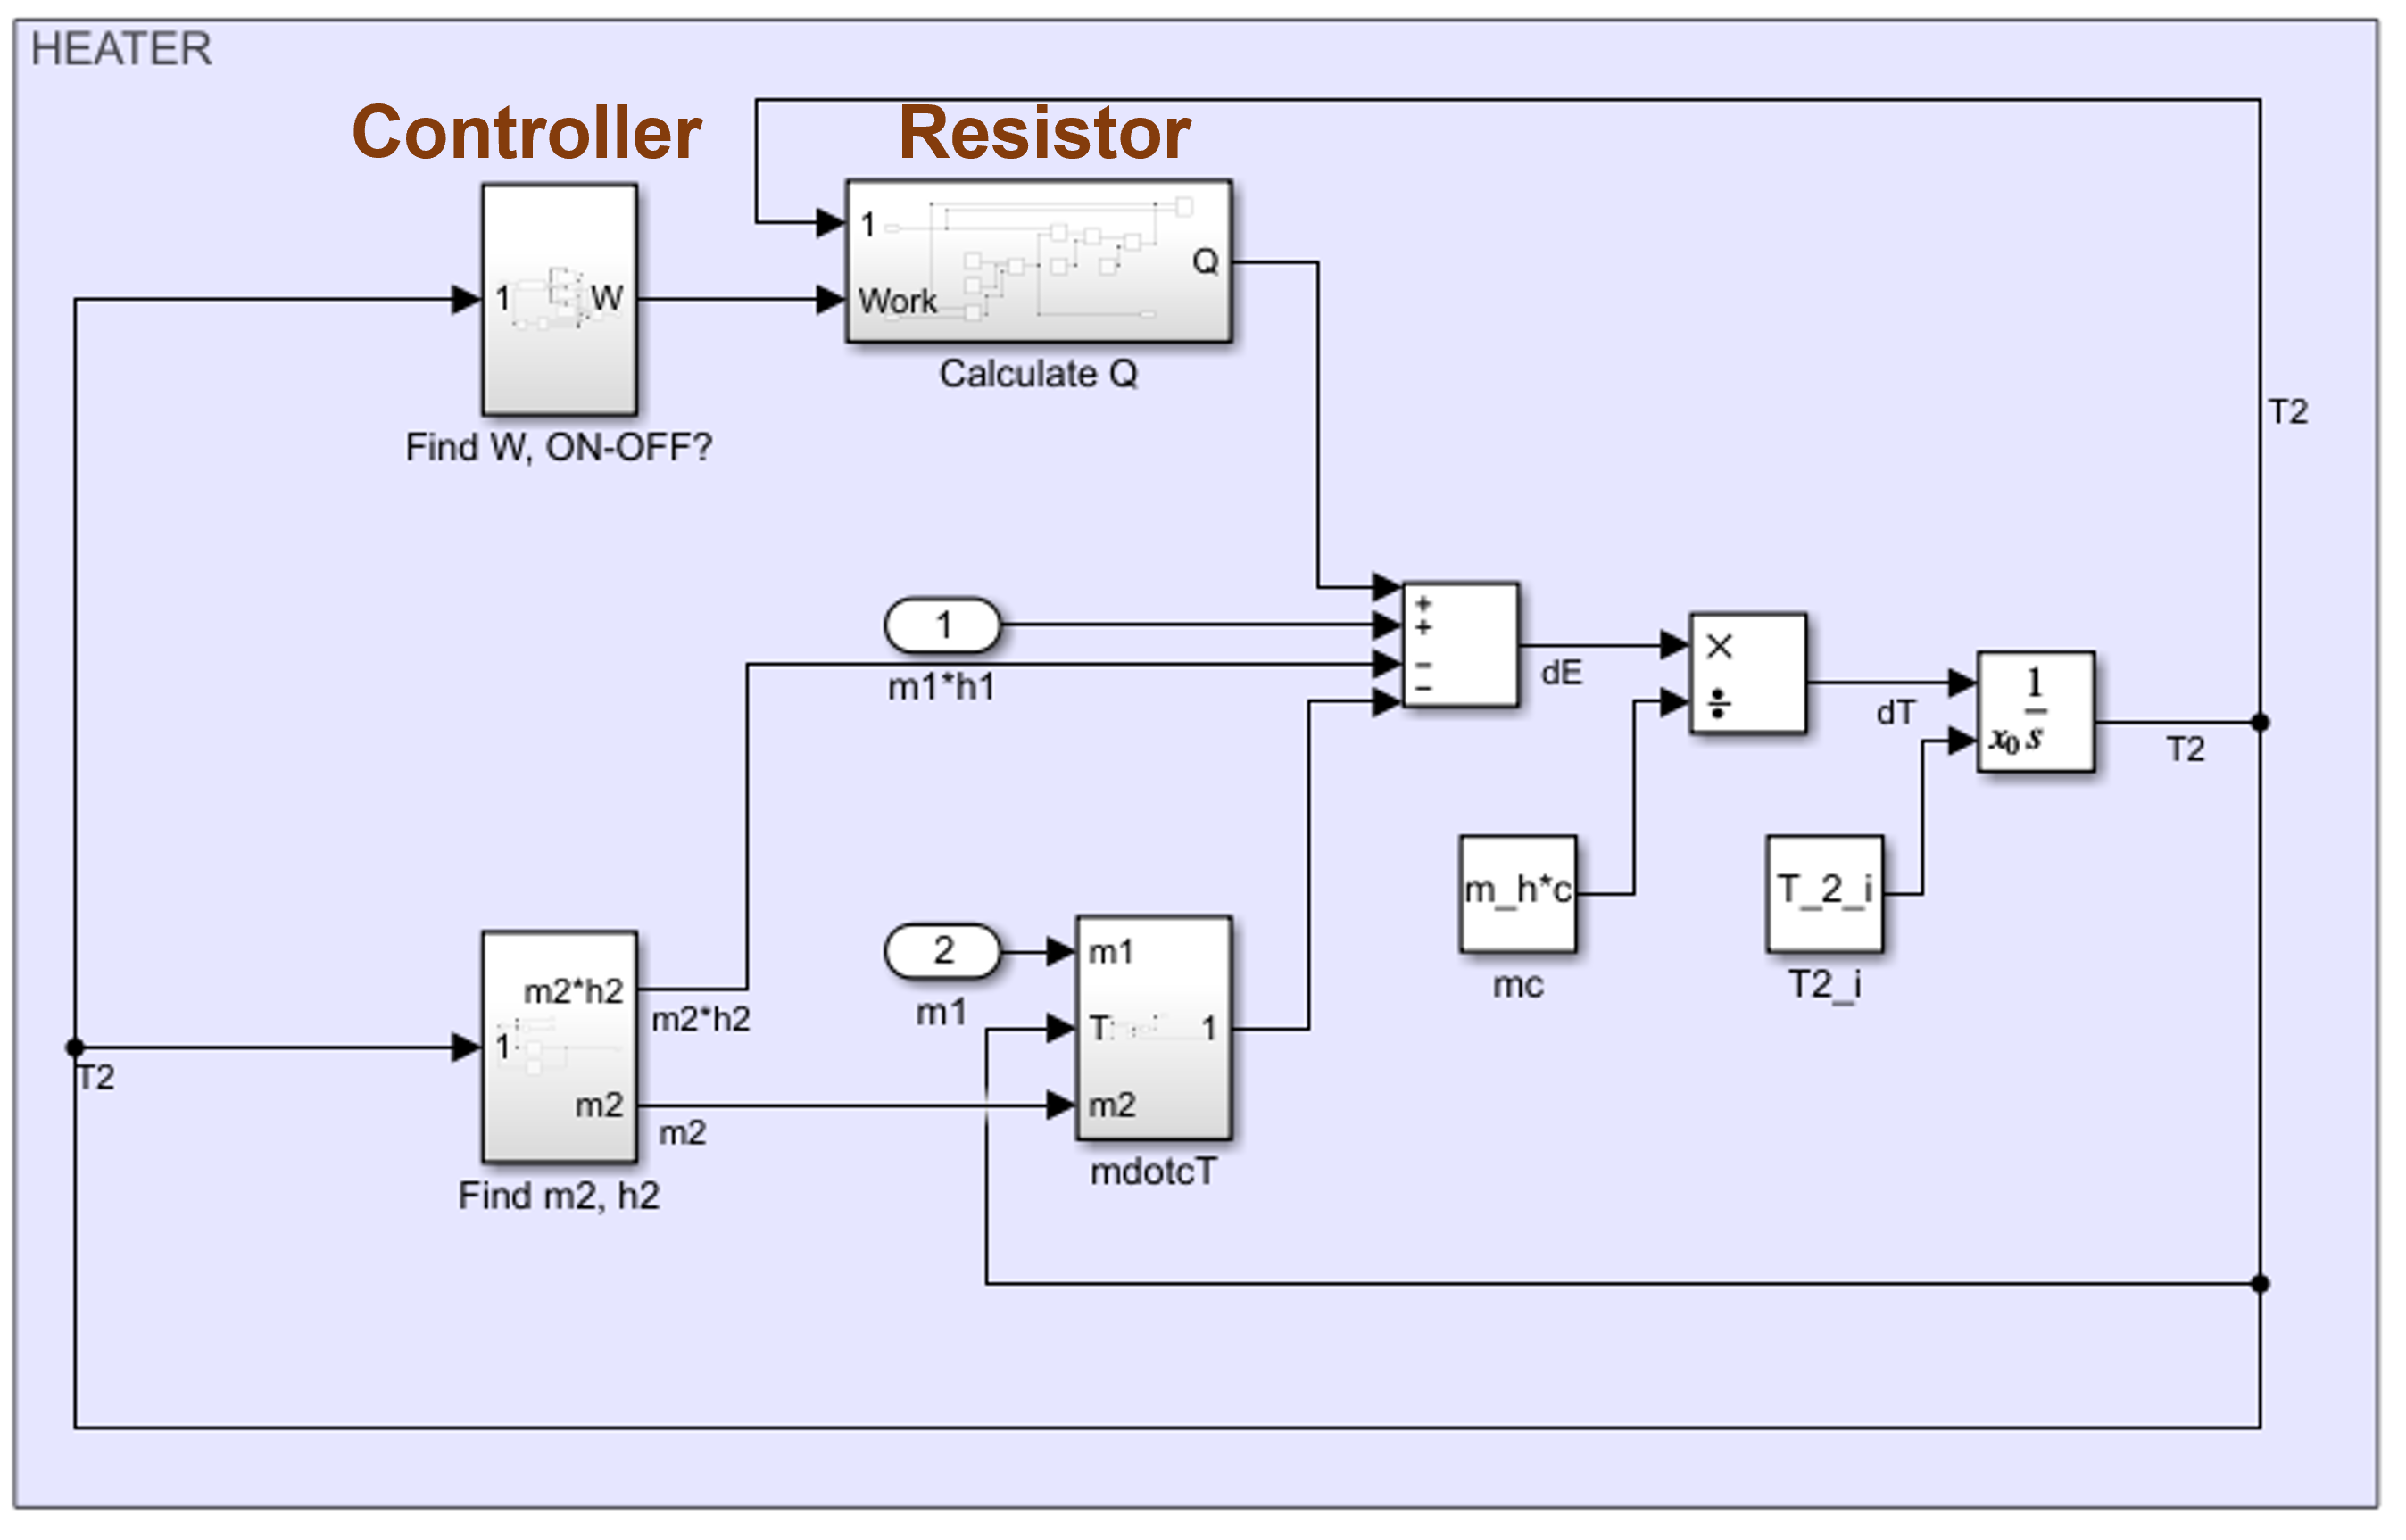
\includegraphics[width=12cm]{images/heater.png}
    \caption{Heater Simulink model.}
    \label{fig:heater}
\end{figure}

\par
In order to calculate the mass flow rate and mass ($\dot{m_{2}}$ and $m_{2}$) inside the heater, volume, and density are required according to Equations \ref{eqn:mass} and \ref{eqn:massflow}. 

\begin{equation}
    \label{eqn:massflow}
    \dot{m} = \rho * \upsilon
\end{equation}
\begin{equation}
    \label{eqn:mass}
    m= \rho * V
\end{equation}

\par
The approximate value of the heater's volume is calculated by on-site measurements and it is equal to $v_{h} = 0.29 m^2$. The density of the oil changes according to the instant temperature. To account for this change, a lookup table is entered into the Simulink model, which determines the density of the oil and makes linear interpolation if necessary. Specific heat ($c_{2}$) and enthalpy values ($h_{1}$ and $h_{2}$) are also determined by a lookup table since it also changes with temperature. These tables are provided in Figure \ref{fig:lookup}.

\begin{figure}[h]
    \begin{minipage}{.5\textwidth}
        \centering
        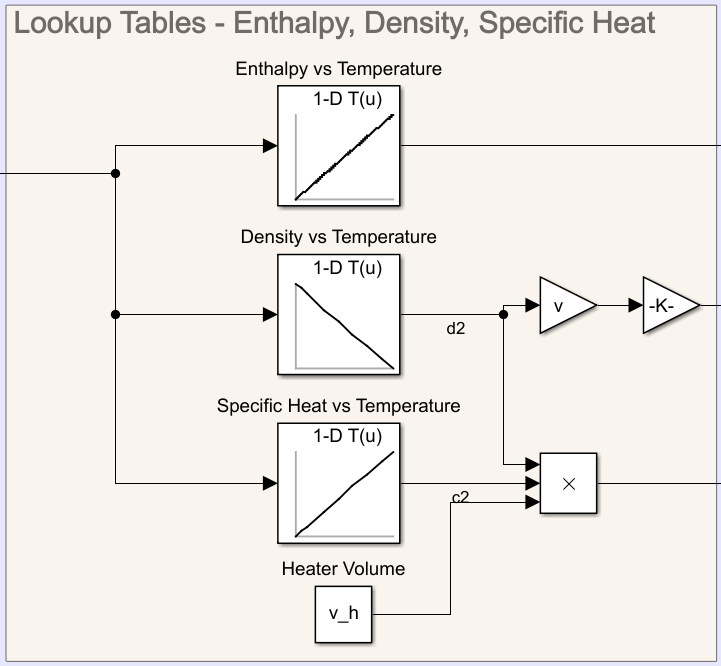
\includegraphics[width=6cm]{images/lookup.png}
        \captionof{figure}{Lookup tables Simulink model.}
        \label{fig:lookup}
    \end{minipage}
    \begin{minipage}{.4\textwidth}
        \centering
        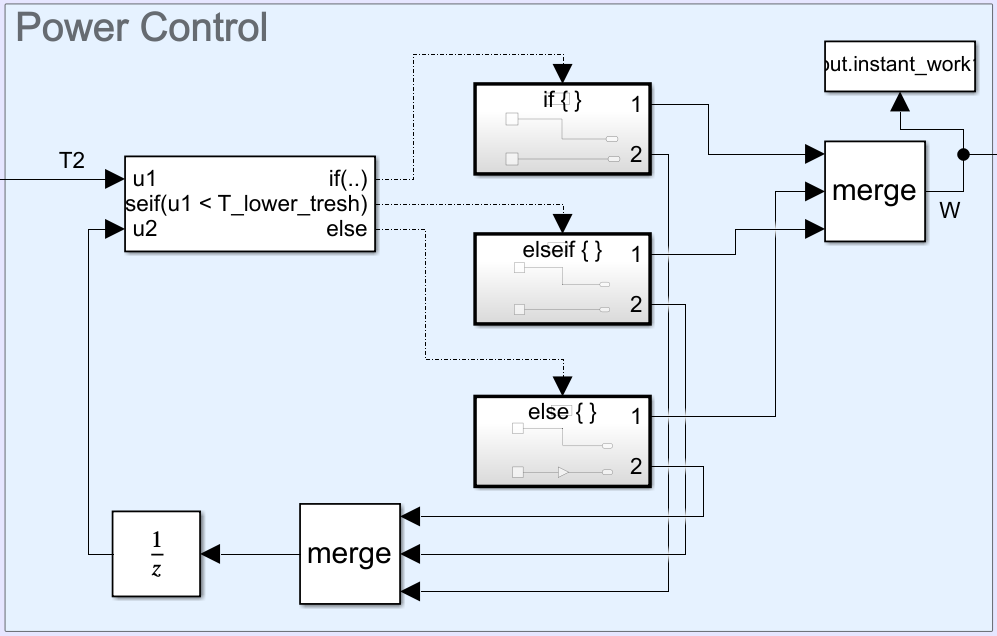
\includegraphics[width=7cm]{images/power.png}
        \captionof{figure}{Power control Simulink model.}
        \label{fig:power}
    \end{minipage}
\end{figure}

\par
Heat transferred to the oil ($Q$) is determined by carrying out the heat transfer calculations between the resistor and oil. 100 kW of electrical power is given to the resistor causing it to dissipate heat. Heat transfer\cite{incropera} to the oil from the resistor is calculated by Equation \ref{eqn:Q}.

\begin{equation}
    \label{eqn:Q}
    Q = UA(T_{r} - T_{2})
\end{equation}

\begin{equation}
    \label{eqn:R}
    \frac{dT_{r}}{dt} = \frac{1}{m_{r}c_{r}}(W - Q) 
\end{equation}

\par
Resistor's temperature ($T_{r}$) is obtained by solving the differential equation given by Equation \ref{eqn:R}. In this equation, the value of the power changes from 0 to 100 kW according to the state of the controller. When the temperature of the oil at the heater exit exceeds an upper threshold, the power is off; when it falls under a lower threshold, the power is on. This behavior is enabled by using if-action blocks of Simulink, as seen in Figure \ref{fig:power}.

\par
Previously mentioned thresholds are determined in a Matlab script and fed to the Simulink model according to the set temperature ($T_{set}$). Not only the thresholds but also the initial values for integral blocks are specified accordingly. Set temperature can be chosen by the user in the same Matlab script with the interface shown in Figure \ref{fig:user}.

\begin{figure}[h]
    \centering
    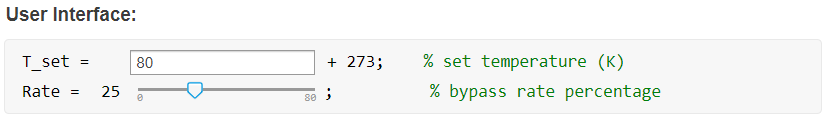
\includegraphics[width=12cm]{images/userinterface.png}
    \caption{Matlab user interface.}
    \label{fig:user}
\end{figure}

In Figure \ref{fig:resistor}, the heat transfer from the resistor to oil is shown in a simplified manner. It is entered into Simulink as shown in Figure \ref{fig:resistorsim}.

\begin{figure}[h]
    \begin{minipage}{.5\textwidth}
        \centering
        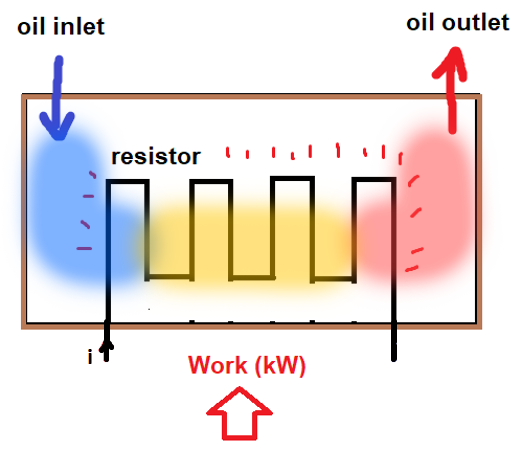
\includegraphics[width=6cm]{images/resistor.png}
        \captionof{figure}{Resistor schematic.}
        \label{fig:resistor}
    \end{minipage}
    \begin{minipage}{.4\textwidth}
        \centering
        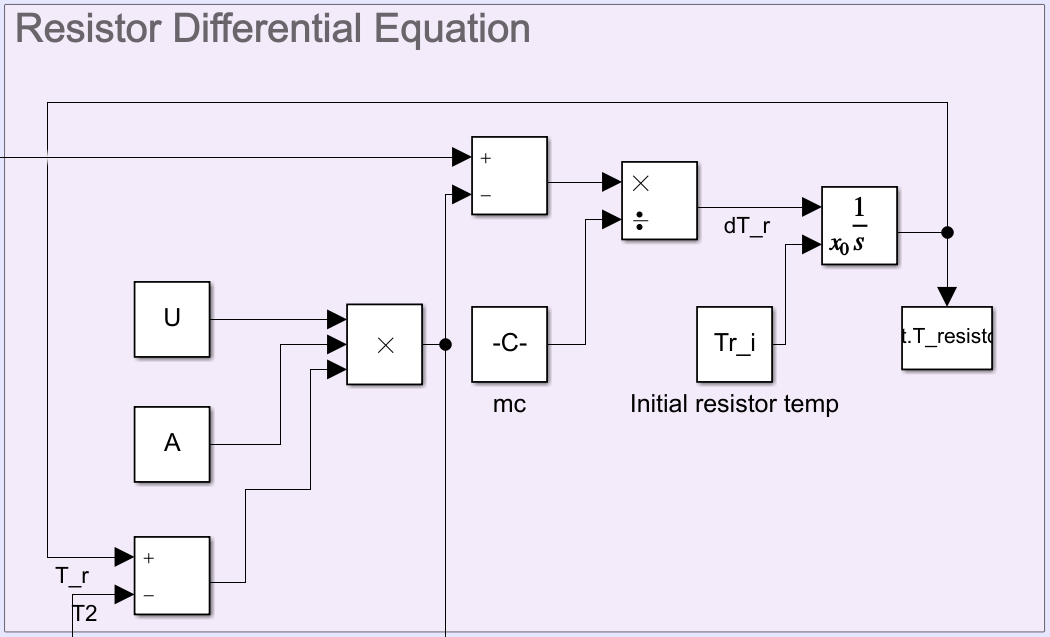
\includegraphics[width=7cm]{images/resistorsim.png}
        \captionof{figure}{Resistor Simulink model.}
        \label{fig:resistorsim}
    \end{minipage}
\end{figure}

\par
Figure \ref{fig:control} shows the temperature variations of the resistor, oil, and on-off status of the controller as input work. 

\par
Also, in Figure \ref{fig:energyflow}, the energy flow in this system can be seen clearly. Electrical energy is transformed into internal energy in the resistor. Then the oil's temperature is increased by the resistor, and finally, in the evaporator, R134A is heated up.


All parameters are found to solve for the temperature at the heater exit except for the resistor's heat transfer coefficient, surface area, mass, and specific heat. These four parameters are treated as two free variables as $UA$ and $m_{r}c_{r}$. These two variables are optimized to give minimum root-mean-square error in Section \ref{training}.

\begin{figure}[H]
    \centering
    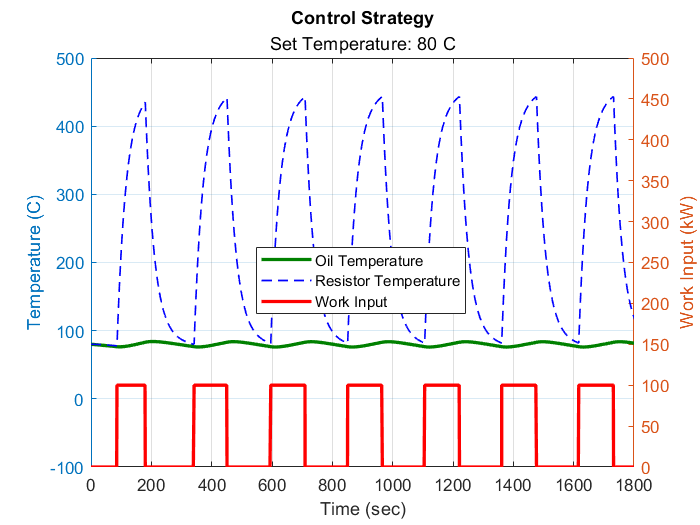
\includegraphics[width=11cm]{images/control_strategy.png}
    \caption{Temperature variations with control strategy.}
    \label{fig:control}
\end{figure}

\begin{figure}[H]
    \centering
    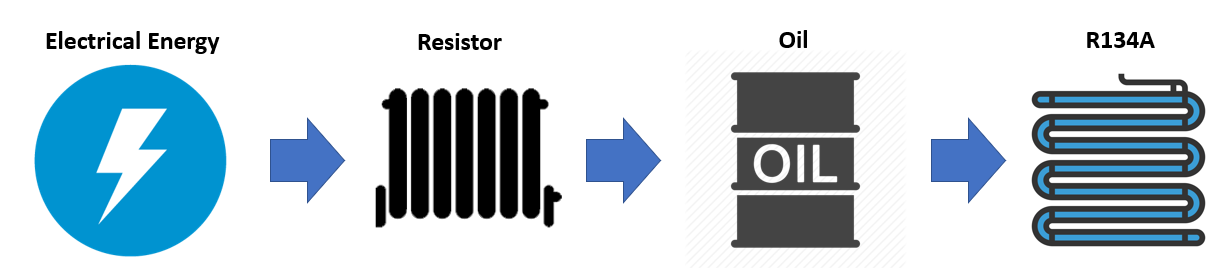
\includegraphics[width=14cm]{images/energyflow.png}
    \caption{Energy flow through the system.}
    \label{fig:energyflow}
\end{figure}

\subsection{Evaporator}
The evaporator model is very similar to the heater model in many respects. Parameters for the evaporator are provided in Table \ref{tab:evaporator}.

\begin{table}[h]
    \centering
    \caption{Evaporator parameters.}
    \label{tab:evaporator}
    \begin{tabular}{|c|c|c|}
        \hline
        \textbf{Symbol} & \textbf{Property}                         & \textbf{Unit} \\
        \hline
        $T_{4}$         & Oil temperature in evaporator             & Kelvin \\
        $m_{4}$         & Oil mass in evaporator                    & kg \\
        $c_{4}$         & Oil's specific heat in evaporator         & kJ/kg*K \\
        $Q_{e}$         & Heat transferred to R134A from oil        & kJ \\
        $\dot{m_{3}}$   & Oil mass flow rate at evaporator entrance & kg/s \\
        $\dot{m_{4}}$   & Oil mass flow rate at evaporator exit     & kg/s \\
        $h_{3}$         & Oil enthalpy at evaporator entrance       & kJ/kg \\
        $h_{4}$         & Oil enthalpy at evaporator exit           & kJ/kg \\
        \hline
    \end{tabular}
\end{table}

The governing differential equation for the evaporator, which is solved to obtain the temperature at the exit of the evaporator, is given in Equation \ref{eqn:evaporator}.

\begin{equation}
    \label{eqn:evaporator}
    \frac{dT_{4}}{dt} = \frac{1}{m_{4}c_{4}}(Q_{e} + \dot{m_{3}}h_{3} - \dot{m_{4}}h_{4})
\end{equation}

In this equation, mass, specific heat, mass flow rates, and enthalpy values are found with the same method provided for the heater using lookup tables. The mass here represents the oil mass inside the evaporator. This mass can be calculated by calculating the volume of the oil inside the evaporator. According to Ertugrul's thesis \cite{altun}, the plates of the evaporator have sinusoidal shapes having a perimeter of 7,64 mm, the area of a sinus wave is $A = 4 mm^2$ per wave, and the heat transfer area is $7.4 m^2$. This means that the total height of the sinusoidal-shaped heat transfer areas must be $h = \frac{7.4 m^2}{7,64 mm}$, and the oil volume inside the evaporator can be calculated as $V = h A = \frac{7.4 m^2}{7,64 mm} 4 mm^2 = 0.387 x 10^{-3} m^3$.

\par
Heat transfer between R134A and oil ($Q_{e}$) is found using experimental values. The temperature of the oil at the inlet and outlet of the evaporator is known. Combining this knowledge with the mass flow rate of the oil, Equation \ref{eqn:Qe} is obtained, which gives the experimental heat transfer amounts for each temperature.

\begin{equation}
    \label{eqn:Qe}
    Q_{e} = \dot{m}c(T_{4} - T_{3})
\end{equation}

Heat transfer value ($Q_{e}$) needs to be updated every second according to the current temperature and for all possible temperature ranges. To do that, experimental values are plotted against temperature, and four different curves are fitted to the plot for four regions. Then, the coefficients of these curves' equations are interpolated for unknown temperature values. This process is explained in Figure \ref{fig:curvefit}.

\begin{figure}[h]
    \centering
    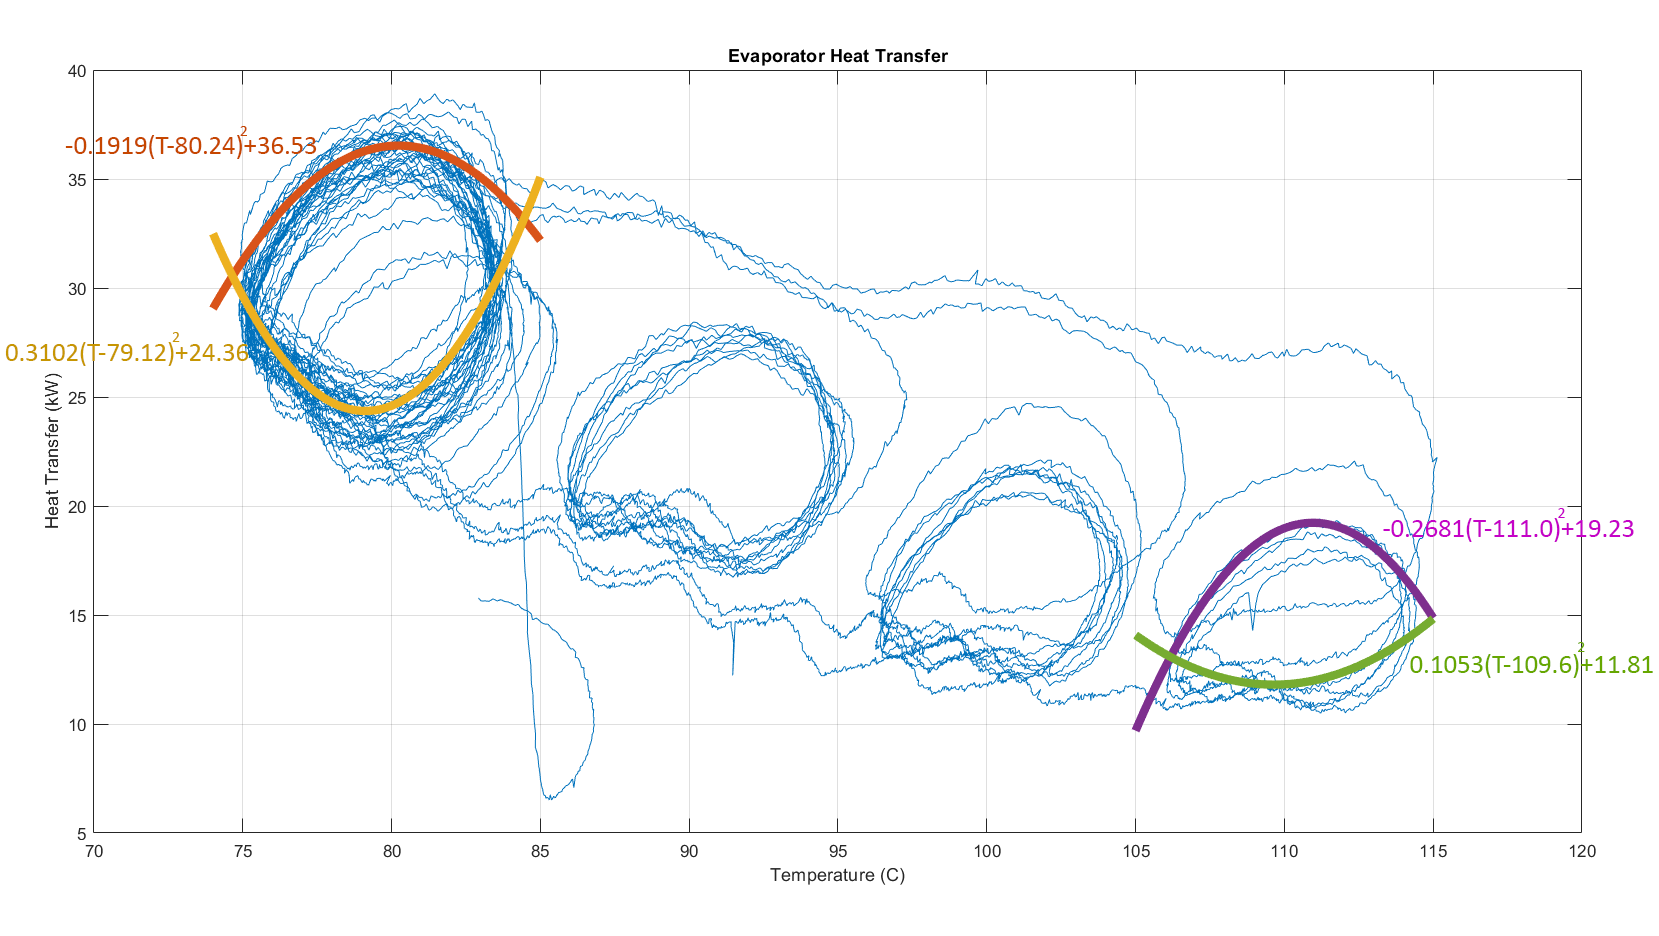
\includegraphics[width=16cm]{images/evaporator_fit.png}
    \caption{Evaporator heat transfer curve fitting to experimental data.}
    \label{fig:curvefit}
\end{figure}

Second-degree polynomials are fitted either in concave or convex format to represent the circular behavior of the data. General format of the polynomial is $Q_{e}(T) = a(T+b)^2+c$. Obtained coefficients are provided in Table \ref{tab:polyfit}.

\begin{table}[h]
    \centering
    \begin{tabular}{|c|c|c|c|}
        \hline
        Type                    & a & b & c \\
        \hline
        Concave, 80 $^\circ C$   & -0.1919 & -80.24 & 36.53 \\
        Concave, 110 $^\circ C$  & -0.2681 & -111.0 & 19.23 \\
        Convex, 80 $^\circ C$   & 0.3102  & -79.12 & 24.36 \\
        Convex, 110 $^\circ C$  & 0.1053  & -109.6 & 11.81 \\
        \hline
    \end{tabular}
    \caption{Coefficients of fitted polynomials.}
    \label{tab:polyfit}
\end{table}

\subsection{Tank}
The tank acts as a pressure stabilizer. The total oil volume in the system changes according to the temperature because temperature changes density. This change in volume is compensated in the tank. Parameters for the tank are provided in Table \ref{tab:tank}.

\begin{table}[h]
    \centering
    \caption{Tank parameters.}
    \label{tab:tank}
    \begin{tabular}{|c|c|c|}
        \hline
        \textbf{Symbol} & \textbf{Property}                         & \textbf{Unit} \\
        \hline
        $T_{1}$         & Oil temperature in tank             & Kelvin \\
        $m_{1}$         & Oil mass in tank                    & kg \\
        $c_{1}$         & Oil's specific heat in tank         & kJ/kg*K \\
        $Q_{loss}$      & Total heat loss in the system       & kJ \\
        $\dot{m_{4}}$   & Oil mass flow rate at tank entrance & kg/s \\
        $\dot{m_{1}}$   & Oil mass flow rate at tank exit     & kg/s \\
        $h_{4}$         & Oil enthalpy at tank entrance       & kJ/kg \\
        $h_{1}$         & Oil enthalpy at tank exit           & kJ/kg \\
        \hline
    \end{tabular}
\end{table}

Tank is also governed by a similar differential equation provided in Equation \ref{eqn:tank}. 

\begin{equation}
    \label{eqn:tank}
    \frac{dT_{1}}{dt} = \frac{1}{m_{1}c_{1}}(Q_{loss} + \dot{m_{4}}h_{4} - \dot{m_{1}}h_{1})
\end{equation}

Heat loss ($Q_{e}$) represents the total heat loss in the system. Heat loss normally occurs in every part, such as pipes, pump, heater, and evaporator, but it is introduced in the tank for ease of solution. It is also another free variable since it is unknown. 

\section{Training}\label{training}
There are three free variables:
\begin{itemize}
    \item Resistor's overall heat transfer coefficient and surface area: $UA$
    \item Resistor's mass and specific heat: $m_{r}c_{r}$
    \item Total heat loss from the system: $Q_{loss}$
\end{itemize}

Before training the model, experimental data is divided into two parts: one for training and the other for validation. This is because, for the reliability of validation, training data needs to be different from the validation data. This separation is shown in Figure \ref{fig:experimentaldata}.

\begin{figure}[h]
    \centering
    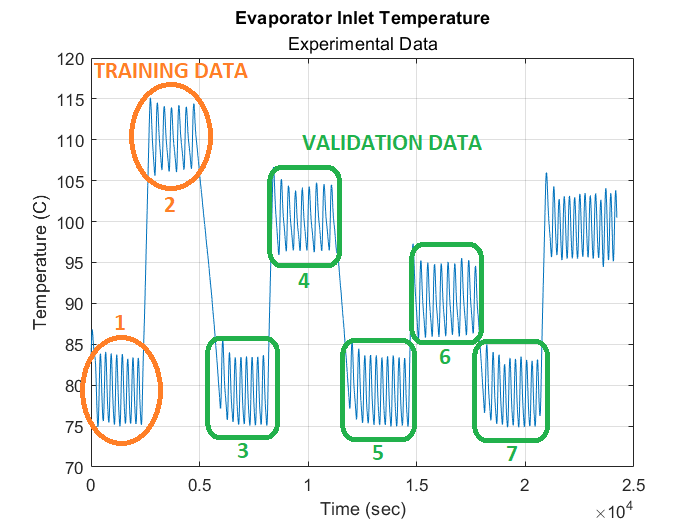
\includegraphics[width=13cm]{images/experimental-data.png}
    \caption{Experimental oil temperature data at evaporator inlet.}
    \label{fig:experimentaldata}
\end{figure}

As seen in Figure \ref{fig:experimentaldata}, in the first section of the experiment temperature is set to 80 $^\circ$C. Then, it is set to 110 $^\circ$C, which is the maximum temperature in the experiment. Oscillation frequency and amplitude change when set temperature is changed. Two far ends are selected as training data to get the nature of these oscillation frequency and amplitude changes.
\par
Many tests are carried out to determine the variables. Comparison plots are created, and RMSE values are calculated for each test. Plots are investigated to prevent under-fitting and over-fitting behaviors because if only the RMSE value is looked at, wrong results may be obtained.
\par
Variables to be determined can be divided into two categories. $UA$ and $m_{r}c_{r}$ are almost constant for all temperature values, and they are assumed as constant. Besides, $Q_{loss}$ significantly changes with the varying temperature, and it accounts for the previously mentioned oscillation frequency and amplitude change with the temperature. That's why at first, two variables $UA$ and $m_{r}c_{r}$ are determined from the test results. Then, the last variable $Q_{loss}$ fits the data both at higher temperatures and lower temperatures.
\par
Final values of the variables:
\begin{itemize}
    \item $UA = 0.27$ \textit{W/K}
    \item $m_{r}c_{r} = 8$ \textit{W/K}
    \item $Q_{loss} = -7.4074*10^{-06}*(T_{set}-110)^4 - 8$ \textit{W}
\end{itemize}

The final version of the plots that are used in the optimization of the variables is provided in Figures \ref{fig:test1} and \ref{fig:test2}.

\begin{figure}[h]
    \begin{minipage}{.5\textwidth}
        \centering
        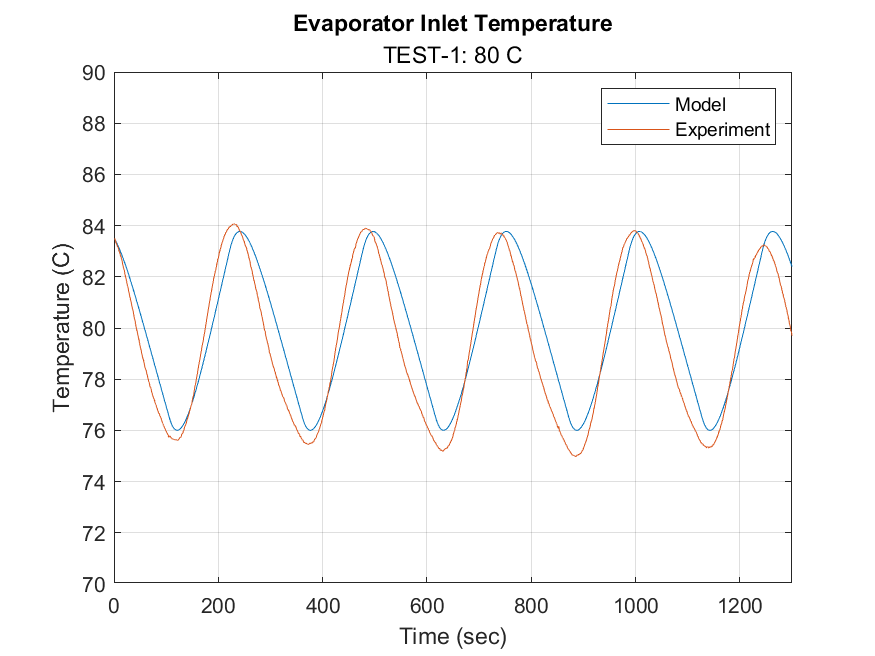
\includegraphics[width=8cm]{images/TEST-1.png}
        \captionof{figure}{Test-1.}
        \label{fig:test1}
    \end{minipage}
    \begin{minipage}{.4\textwidth}
        \centering
        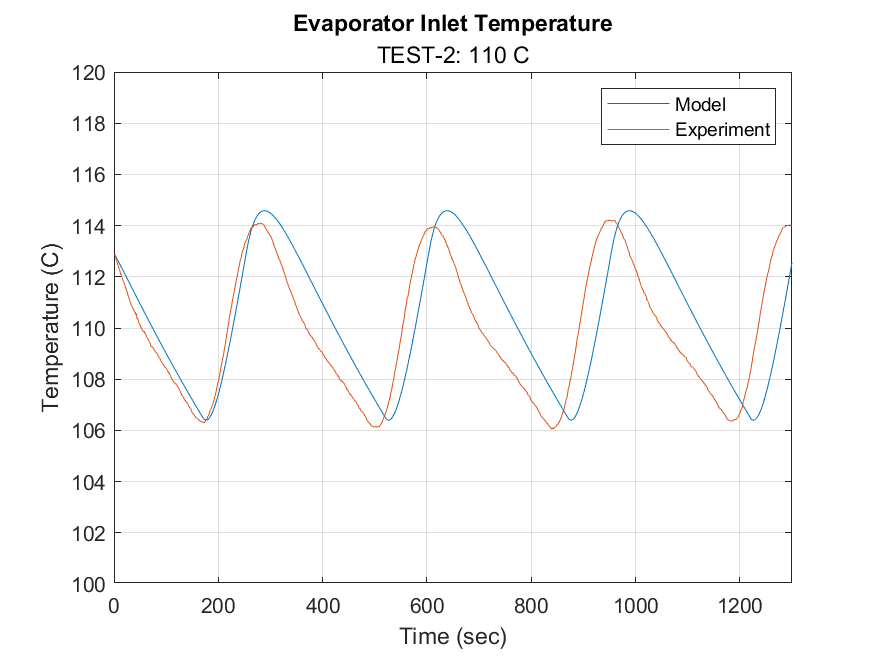
\includegraphics[width=8cm]{images/TEST-2.png}
        \captionof{figure}{Test-2.}
        \label{fig:test2}
    \end{minipage}
\end{figure}


\section{Proposed Solution}

\begin{figure}[H]
    \centering
    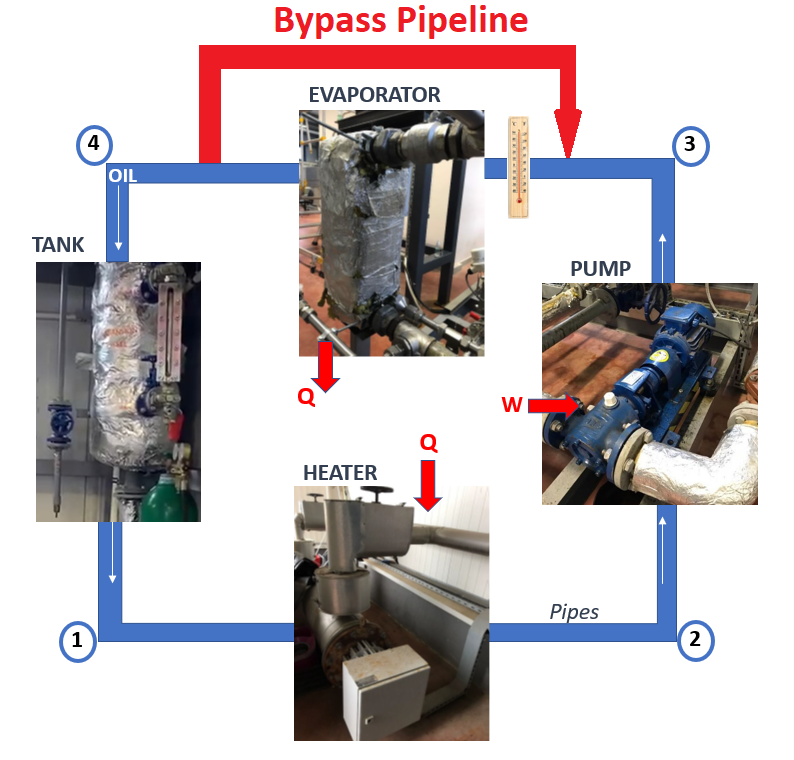
\includegraphics[width=10cm]{images/cycle_v2.png}
    \caption{Oil cycle with suggested method.}
    \label{fig:cycle_v2}
\end{figure}

The main goal of this project is to reduce the oil's temperature oscillations in the evaporator by applying mechanical solutions. A lower oscillation portion of the oil can be mixed with the mainstream oil just before the evaporator inlet. In Figure \ref{fig:cycle_v2}, our suggested method is implemented on the oil cycle.


According to the investigations of the experimental data, it is found that the oil's temperature oscillations are lower at the evaporator exit. Also, there already exists a bypass line between the inlet and exit of the evaporator. Thus, the proposed solution is feeding back the exiting oil to the inlet of the evaporator via this bypass line. This method is implemented in Simulink as seen in Figure \ref{fig:oldandnew}.

\bigskip

\begin{figure}[H]
    \centering
    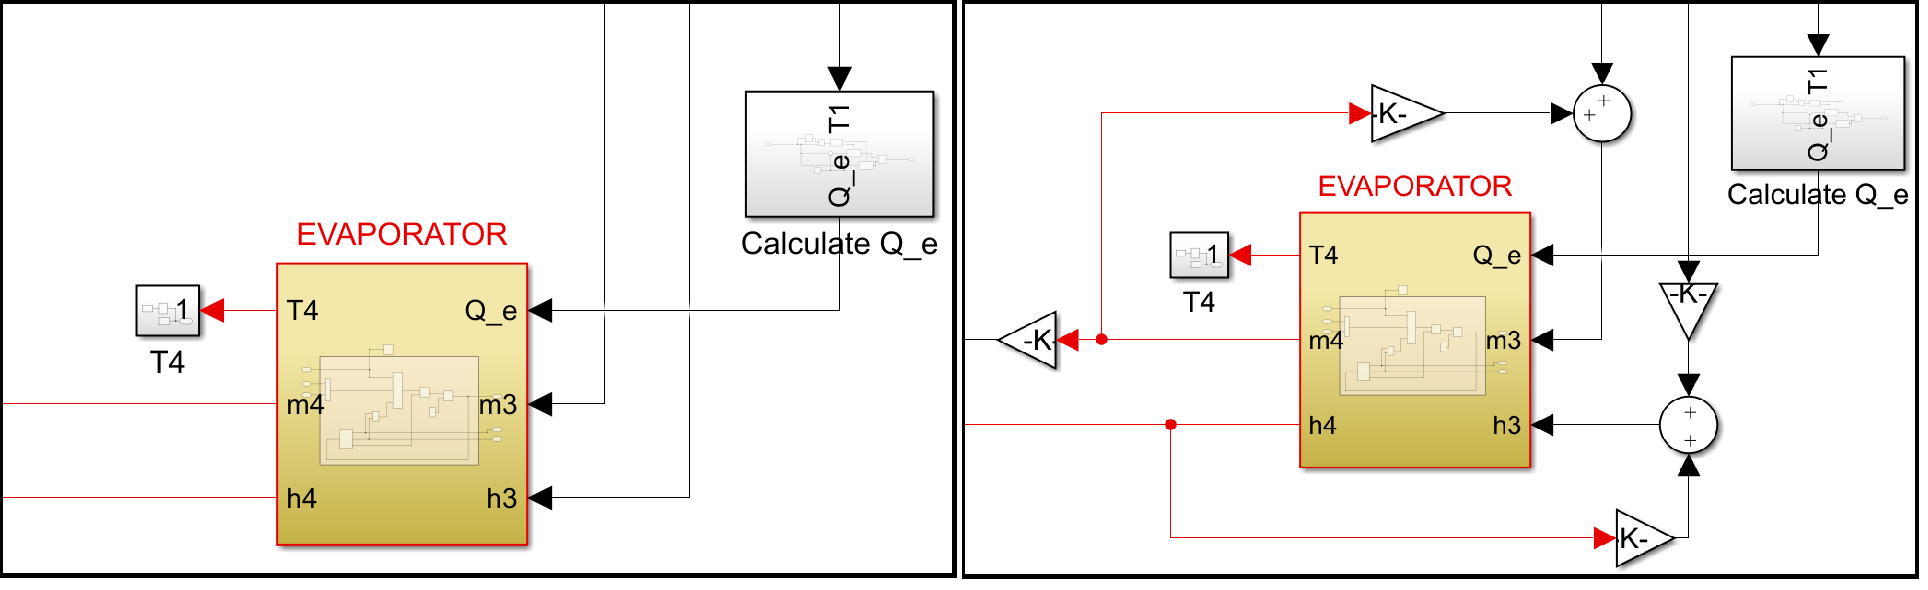
\includegraphics[width=14cm]{images/oldandnew.png}
    \caption{Evaporator model before and after the proposed solution is implemented.}
    \label{fig:oldandnew}
\end{figure}
    \chapter{Experimental Setup}

There are some crucial components needed in order to carry out the experiment of the proposed solution. Note that in the oil cycle part of ORC, there is an already installed bypass line. This bypass line can be used to reduce the cost of implementing the proposed solution.

\begin{enumerate}
    \item First of all, a pump is needed to establish a flow in the reverse direction of the cycle.
    \item Second, a check valve is needed to ensure fluid flow only in one direction in the bypass line.
    \item Third, a 3-way valve and an actuator must be employed at the entrance of the bypass line to control the mass flow rate that will flow inside the bypass pipeline
    \item Lastly, a power source for the actuator is needed.
\end{enumerate}

\section{Concept Setup of the Proposed Solution}

\begin{figure}[H]
		\centering
		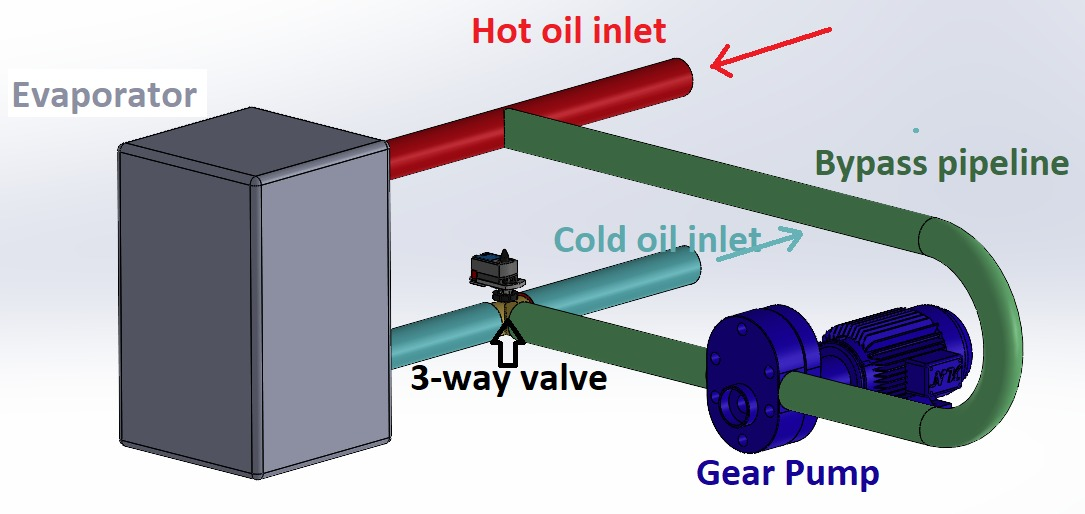
\includegraphics[width=0.8\textwidth]{images/tasarim.jpg}
		\caption[Concept Setup of the Proposed Solution]{Concept Setup of the Proposed Solution}
		\label{concept} 
\end{figure} 

The bypass pipeline connects the exit of the evaporator to the inlet of the evaporator. Since there is a height difference between the inlet and exit of the evaporator and there is a pressure loss inside the evaporator, it is not possible to constitute a flow from exit to inlet without a pump. Therefore, an appropriate pump is needed to be installed in order to employ a reverse flow. There are some crucial criteria for the pump. The pump must endure temperatures as high as $140^\circ$. Additionally, the pump must not corrode by oil. Generally, in high-temperature oil applications, gear pumps that are capable of enduring high-temperature oil are used. The head a gear pump provides is not much important since there is a small height difference between the inlet and the exit, and the pressure loss inside the evaporator is negligibly low, according to Ertugrul's thesis. A gear pump is approximately 5500 TLs.

\begin{figure}[H]
		\centering
		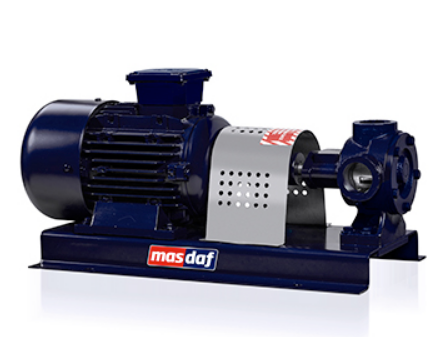
\includegraphics[width=0.5\textwidth]{images/pump.png}
		\caption[A Gear Pump]{A Gear Pump}
		\label{pump} 
\end{figure} 

Moreover, a proper check valve must be installed as well to ensure a one-direction-only flow. The same criteria are valid for the check valve: the valve must endure high-temperature oil. For this use, a disc type of check valve made up of stainless steel can be installed since it can endure high temperatures and will not corrode because of its material. This type of check valve is around 500 TLs.

\begin{figure}[H]
		\centering
		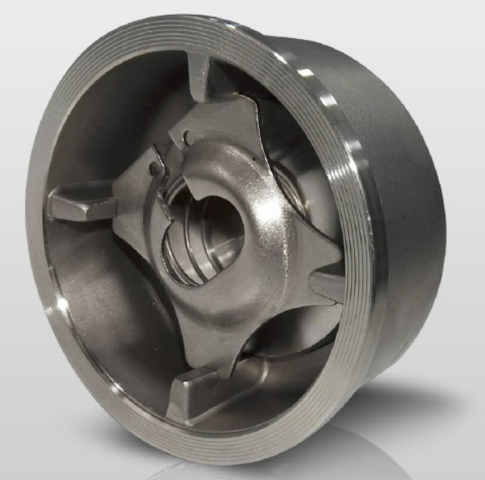
\includegraphics[width=0.3\textwidth]{images/valve_2.png}
		\caption[A Disc Check Valve]{A Disc Check Valve}
		\label{valve_2} 
\end{figure} 

Additionally, a 3-way valve will be used to establish an adjustable fluid flow direction. There are a couple of options for the type of 3-way valve, but since there is an available 3-way ball valve in the BURET lab, there is not much reason to purchase a new valve. The available 3-way ball valve is Siemens VB61.50-40 DN50 which is a brass valve with a stainless steel ball. The ball can be rotated by rotating the rectangular-shaped pin above the ball. 

\begin{figure}[H]
		\centering
		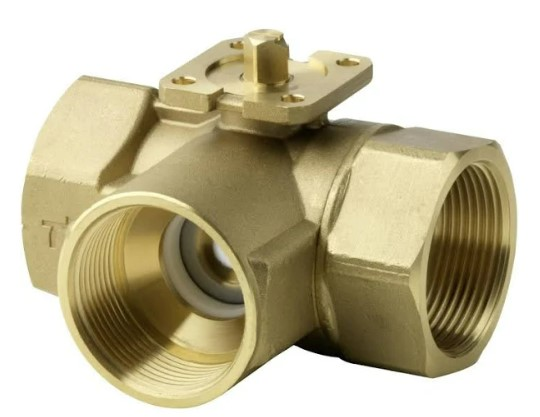
\includegraphics[width=0.3\textwidth]{images/valve.jpg}
		\caption[3-way ball valve]{3-way ball valve}
		\label{valve} 
\end{figure} 

Additionally, an actuator is needed to control the fluid flow direction by rotating the ball inside the valve. There is also an available actuator in the BURET lab, which is Siemens GLB161.9E. The actuator is coherent with the 3-way ball valve, so it can rotate the pin on the valve. Furthermore, there must be a 24V power supply for the actuator to rotate.

\begin{figure}[H]
		\centering
		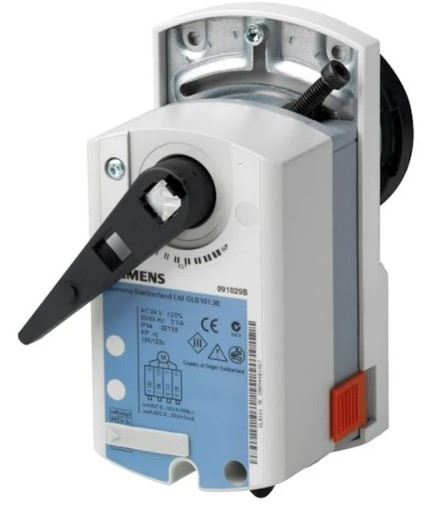
\includegraphics[width=0.3\textwidth]{images/actuator.jpeg}
		\caption[Actuator - Siemens GLB161.9E]{Actuator - Siemens GLB161.9E}
		\label{actuator} 
\end{figure} 

\par
In Table \ref{tab:components}, the components required for applying our solution method are listed with the corresponding costs.

%% TABLE
\begin{table}[h]
    \centering
    \begin{tabular}{|c|c|}
         \hline 
         \textbf{Components}    & \textbf{Cost}  \\
         \hline
         Three-way valve        &  4400 TL         \\
         Gear pump              &  5500 TL         \\
         Disc check valve       &  500  TL         \\
         Rotary actuator        &  2300 TL         \\
         \hline
         \textit{Total cost}    &  12700 TL         \\
         \hline
    \end{tabular}
    \caption{Components and costs.}
    \label{tab:components}
\end{table}

Since the bypass pipeline, 3-way ball valve, and actuator are already available, the initial cost of setting this experiment up is around 6000 TLs. Due to the cost limitations, however, a more comprehensive experiment that consists of a pump and a check valve is not done. Instead, our experimental setup will cover controlling an actuator connected to a 3-way ball valve which will control the mass flow rate in the bypass pipeline.

\section{Setup of the Experiment}

The setup of the experiment consists of three main parts, which are a 3-way ball valve, an actuator, and a power supply. There are also some cables, a resistance, and a potentiometer used. The purpose of the experiment was to establish a setup that can control the actuator's angle, which represents how much the ball valve supplies fluid to the bypass pipeline. The actuator has four cables connected to it which are the power inlet, the ground, the control, and the feedback cables. A 24V power supply is added to the setup to power the actuator. The power inlet and ground cables of the actuator are connected to this power supply.

By controlling the voltage across the control and feedback cables, the actuator can be rotated between $0^\circ$  which represents that the ball valve is closed, meaning there will be no flow to the bypass pipeline, and $90^\circ$ which represents the ball valve closed the inlet of the evaporator and fully opened the bypass pipeline. Since a closed evaporator inlet is not desired in the experiment, the actuator should never be rotated to $90^\circ$.

To control the voltage across the control and feedback cables, a simple electronic circuit must be established. The rotation of the actuator is related to the voltage difference between the feedback and control cables. If the feedback's voltage is more than the control cables, then the actuator rotates toward $90^\circ$. If the voltage across the control is more than the feedback's, then the actuator rotates toward $0^\circ$. The actuator stops when the voltage across the control and feedback cables are nearly equal to each other. The mechanism of the actuator requires that an adjustable resistance should be placed to control the voltage. Therefore, a potentiometer is placed between the control cable and the ground to establish an adjustable voltage across the control cable. Additionally, the feedback cable must be connected to a resistor before the ground. Otherwise, the voltage across the feedback 
will always be bigger than the control's voltage.

\begin{figure}[H]
		\centering
		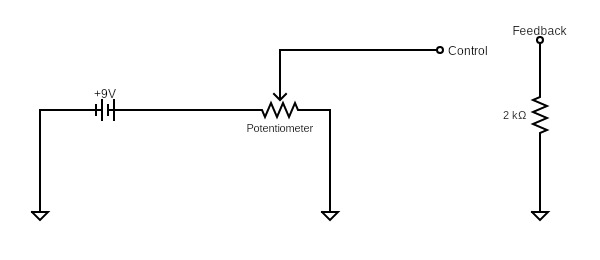
\includegraphics[width=0.7\textwidth]{images/devre.jpg}
		\caption[Circuit Diagram of the Experiment Setup]{Circuit Diagram of the Experiment Setup}
		\label{devre} 
\end{figure}


\begin{figure}[H]
    \centering
    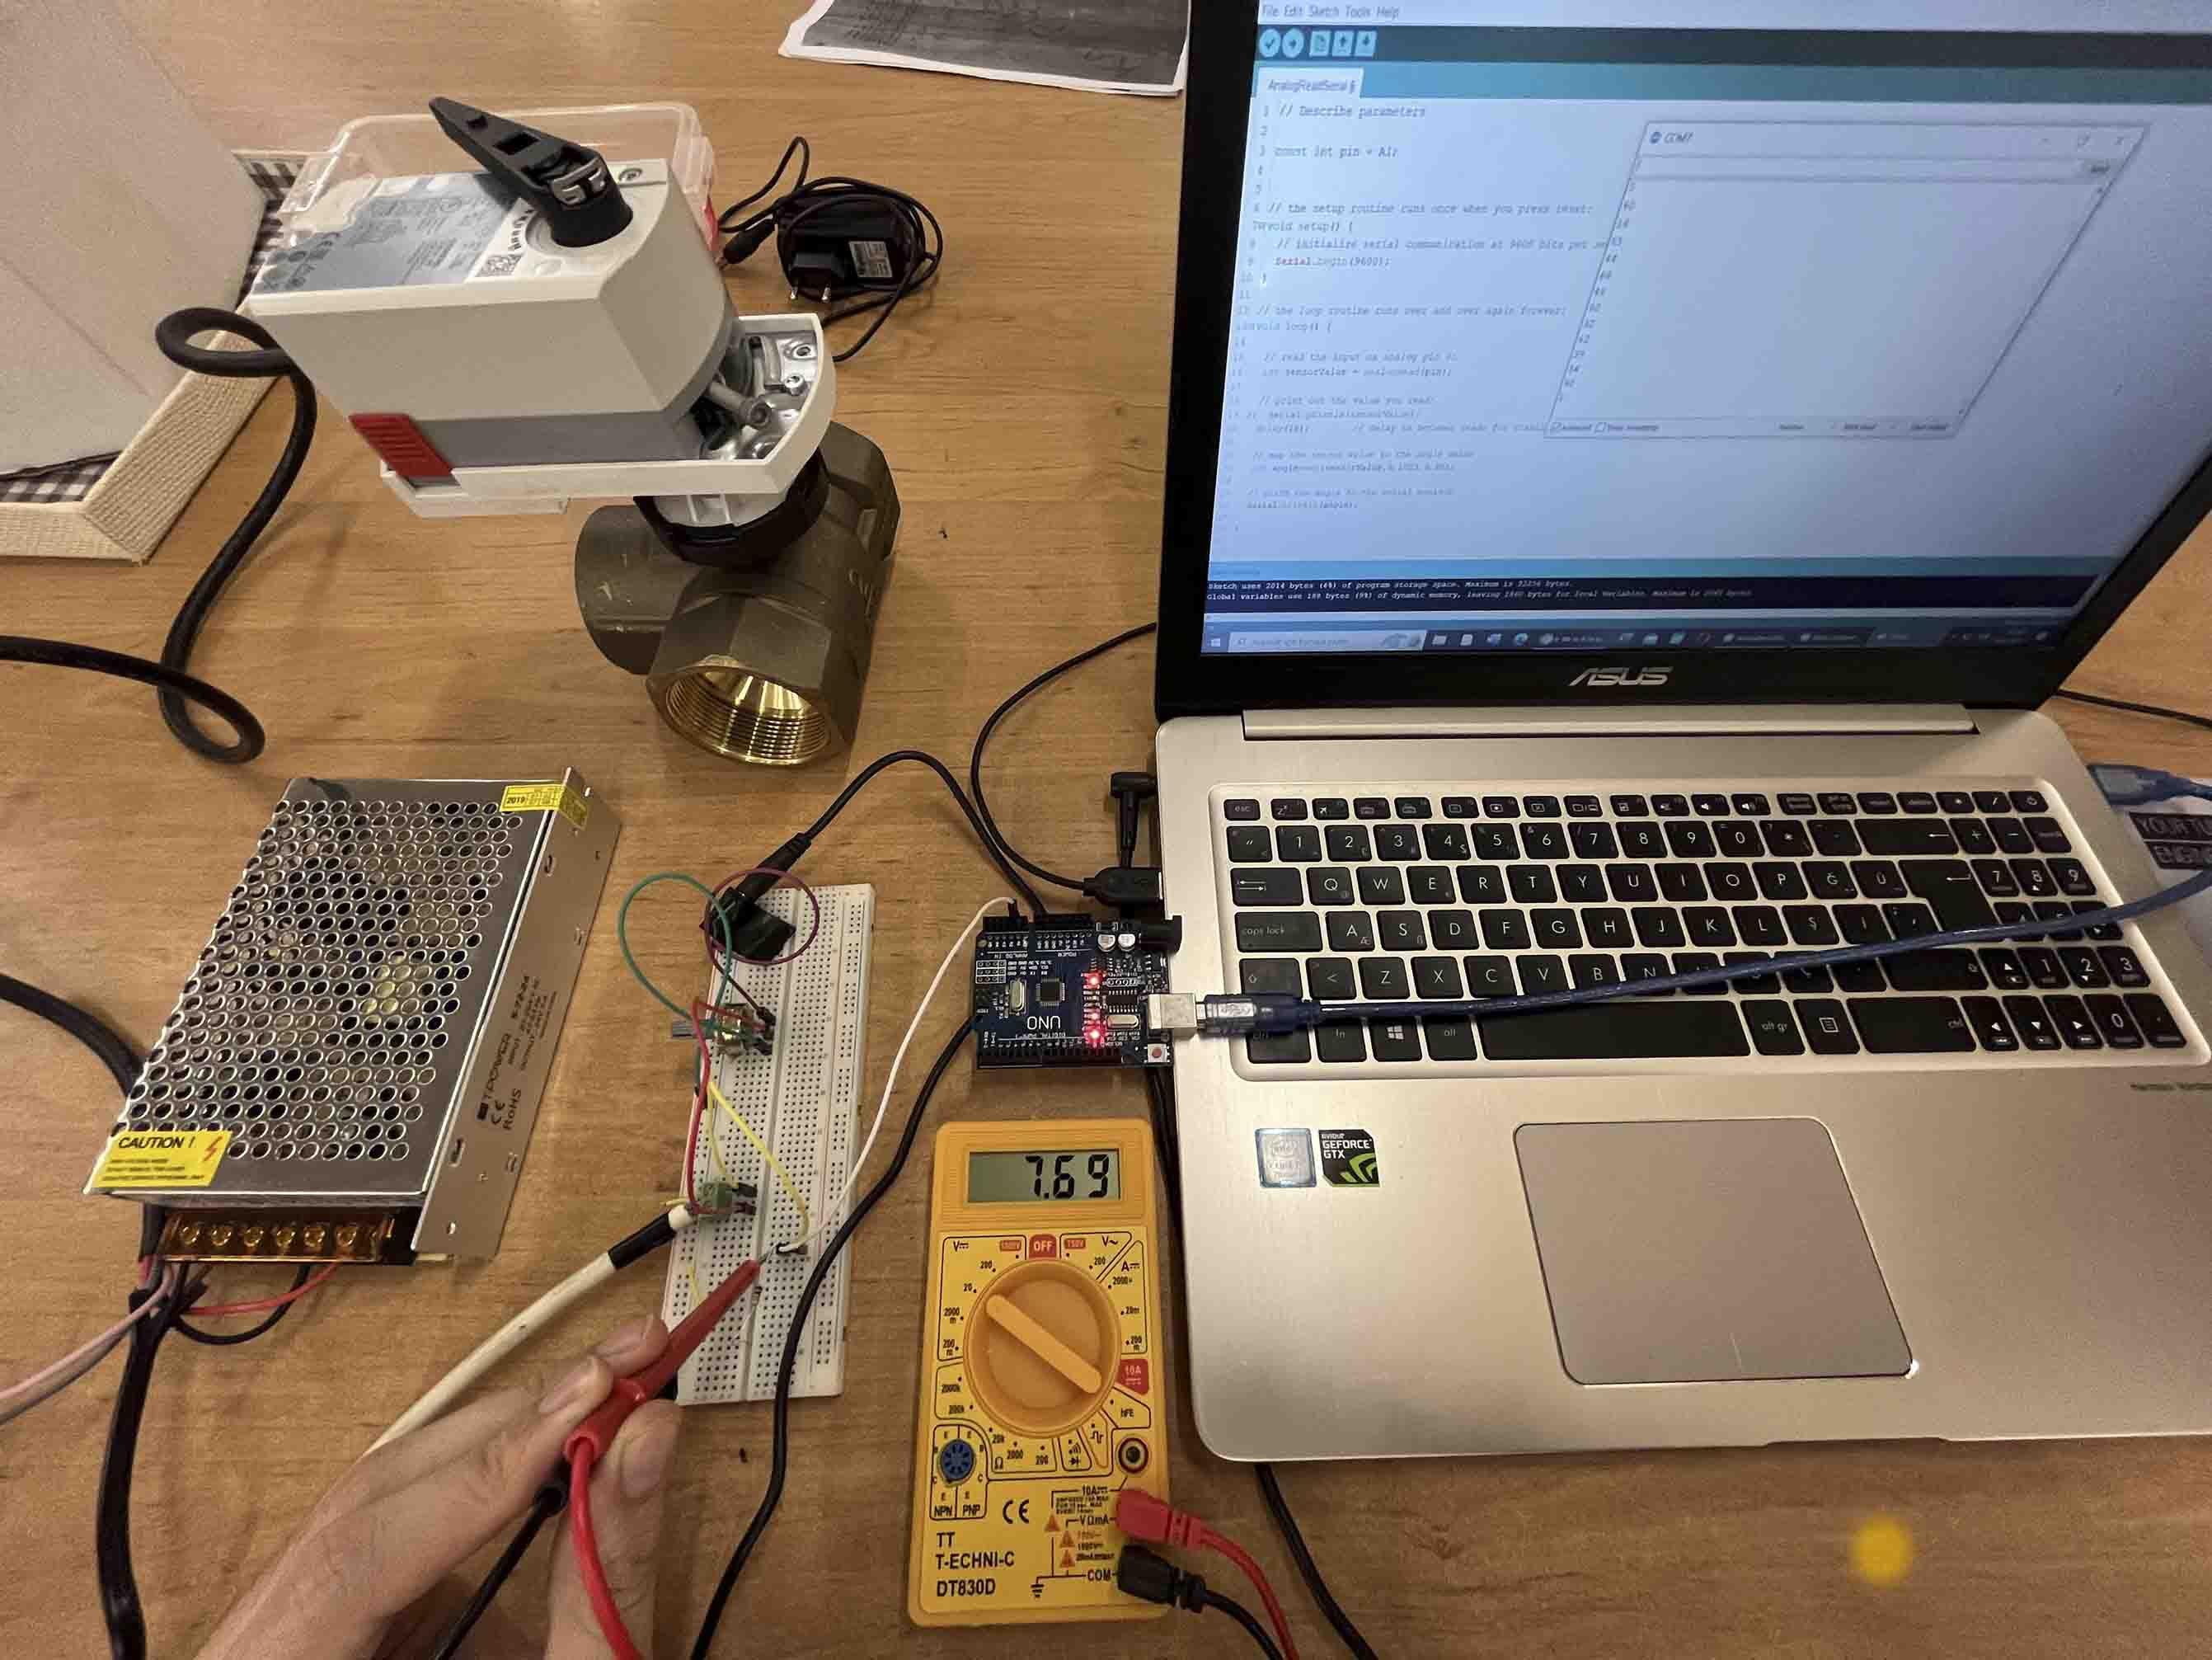
\includegraphics[width=15cm]{images/actuator.jpg}
    \caption{Actuator motor control.}
    \label{fig:actuator}
\end{figure}

\par
In case of a possible real-world implementation, the damper actuator is tested. It is connected to the three-way valve, and then the valve is opened and closed respectively. In order to do that, all connections of the actuator are made. It is connected to a 24V DC power supply, its control signal is connected to a 12V DC power supply, and its voltage is controlled by a 10k potentiometer. The feedback signal is connected to the Arduino's A1 analog input port. The incoming signal is converted to the angle and read from the serial monitor. Several positions are tested, and a video recording is completed during this process.

\par
This damper actuator control setup is shown in Figure \ref{fig:actuator}


    \chapter{Results \& Discussion}

\section{Validation}
Variables are determined in the previous section. In this section, by using these variables and the model, five different plots regarding the different set temperatures and trials are generated to compare the model's results with the experimental data. 
\par
Validation plots are provided below in Figures \ref{fig:test3}, \ref{fig:test4}, \ref{fig:test5}, \ref{fig:test6} and \ref{fig:test7}.

\begin{figure}[h]
    \begin{minipage}{.5\textwidth}
        \centering
        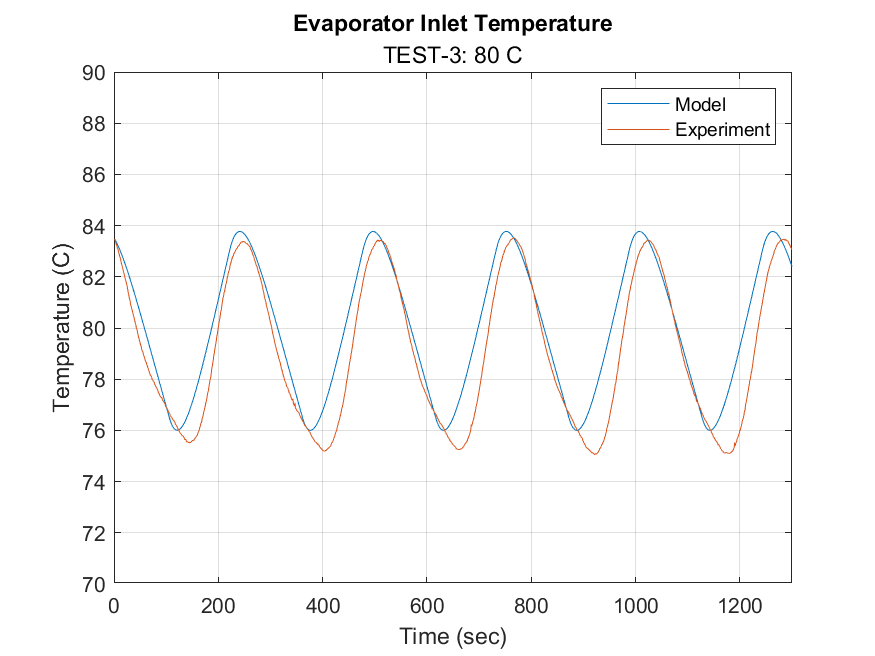
\includegraphics[width=8cm]{images/TEST-3.png}
        \captionof{figure}{Test-3.}
        \label{fig:test3}
    \end{minipage}
    \begin{minipage}{.4\textwidth}
        \centering
        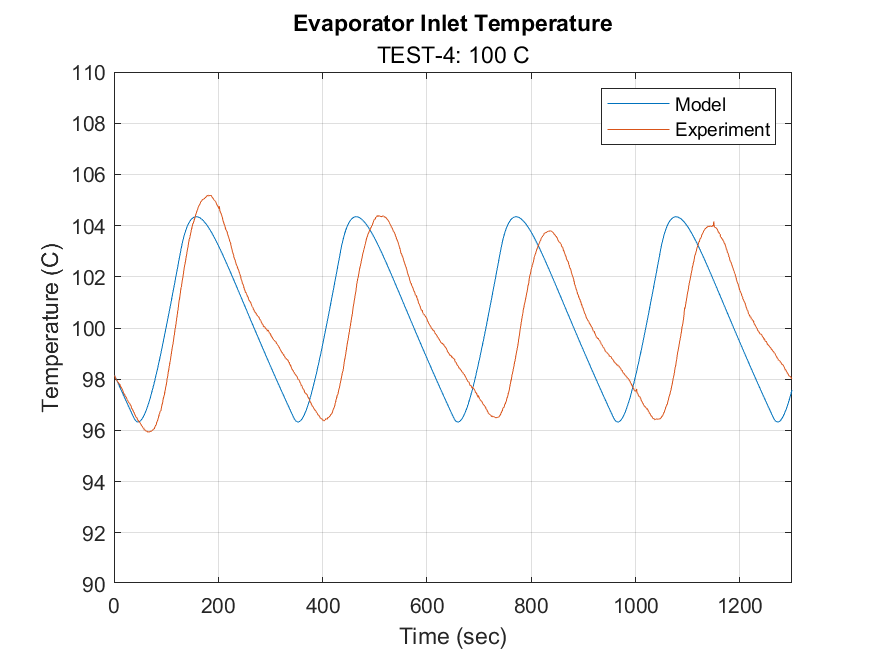
\includegraphics[width=8cm]{images/TEST-4.png}
        \captionof{figure}{Test-4.}
        \label{fig:test4}
    \end{minipage}
\end{figure}

\bigskip

\begin{figure}[h]
    \begin{minipage}{.5\textwidth}
        \centering
        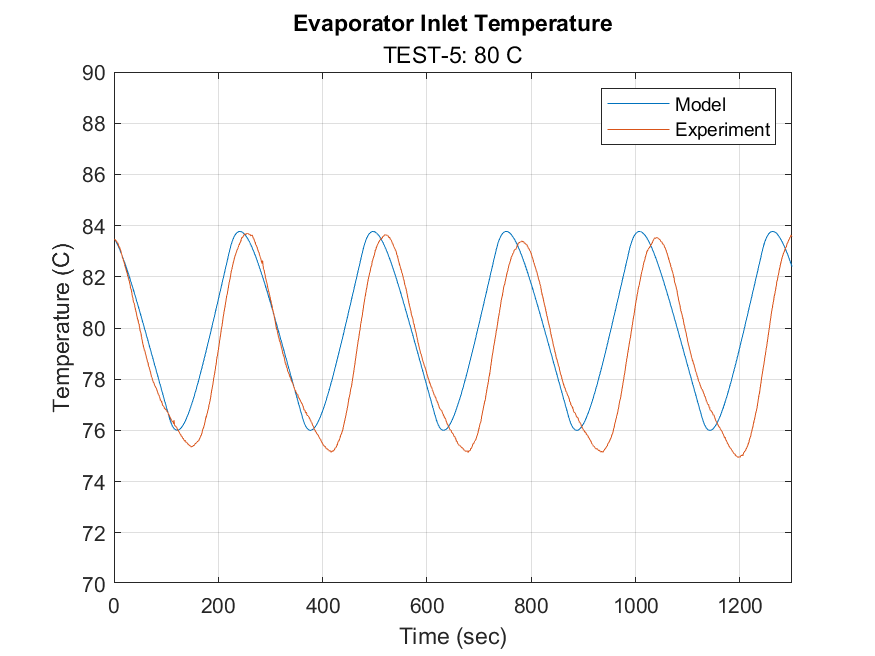
\includegraphics[width=7.2cm]{images/TEST-5.png}
        \captionof{figure}{Test-5.}
        \label{fig:test5}
    \end{minipage}%
    \begin{minipage}{.4\textwidth}
        \centering
        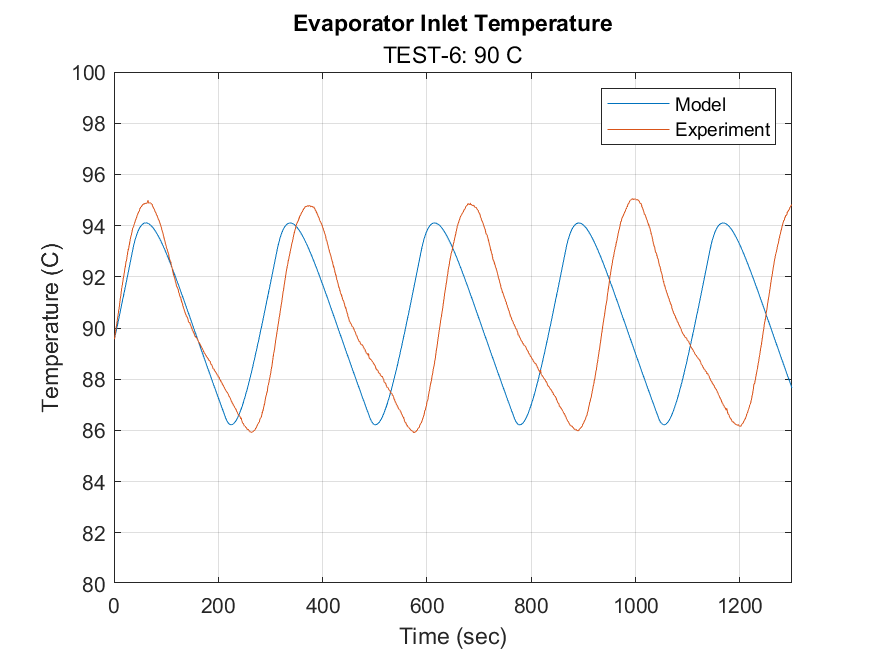
\includegraphics[width=7.2cm]{images/TEST-6.png}
        \captionof{figure}{Test-6.}
        \label{fig:test6}
    \end{minipage}
\end{figure}

\bigskip

\begin{figure}
    \centering
    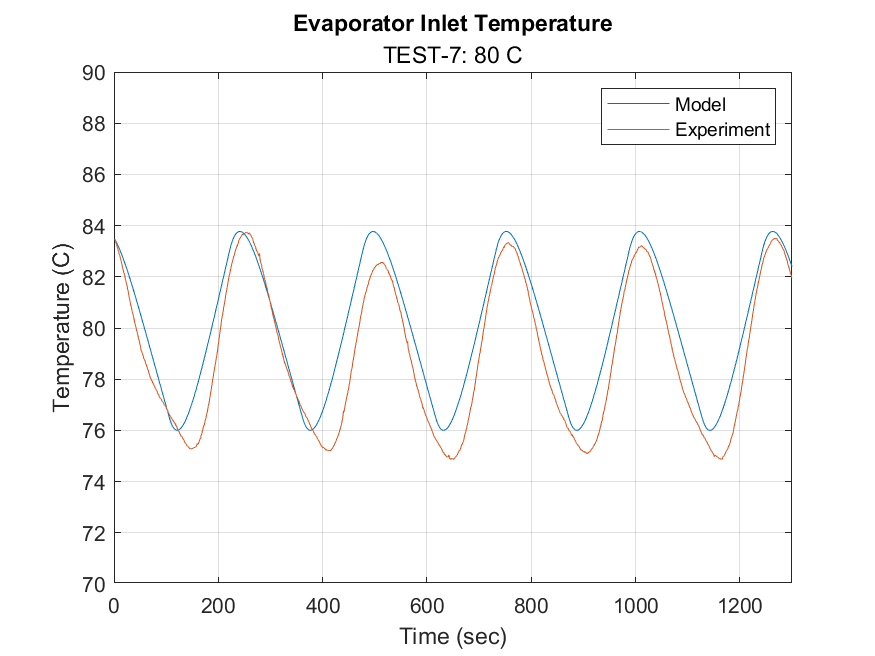
\includegraphics[width=7.2cm]{images/TEST-7.png}
    \caption{Test-7.}
    \label{fig:test7}
\end{figure}

As can be seen, the results of the simulations are highly coherent with the experiment results. Tests 3 and 7 show that the model produces better results at low set temperatures, except for test 5. Test 4 and 6 demonstrates that the model data has a slightly low period than the experiment data when the set temperature is high.

\section{Result of the Bypass Pipeline}

To see if the proposed solution works or not, the model is tested by setting a bypass rate. Then the results are compared with the older results without bypass line usage. The decrease in the oscillation amplitude is measured. The resulting plot is provided in Figure \ref{fig:result}.

\begin{figure}[H]
    \centering
    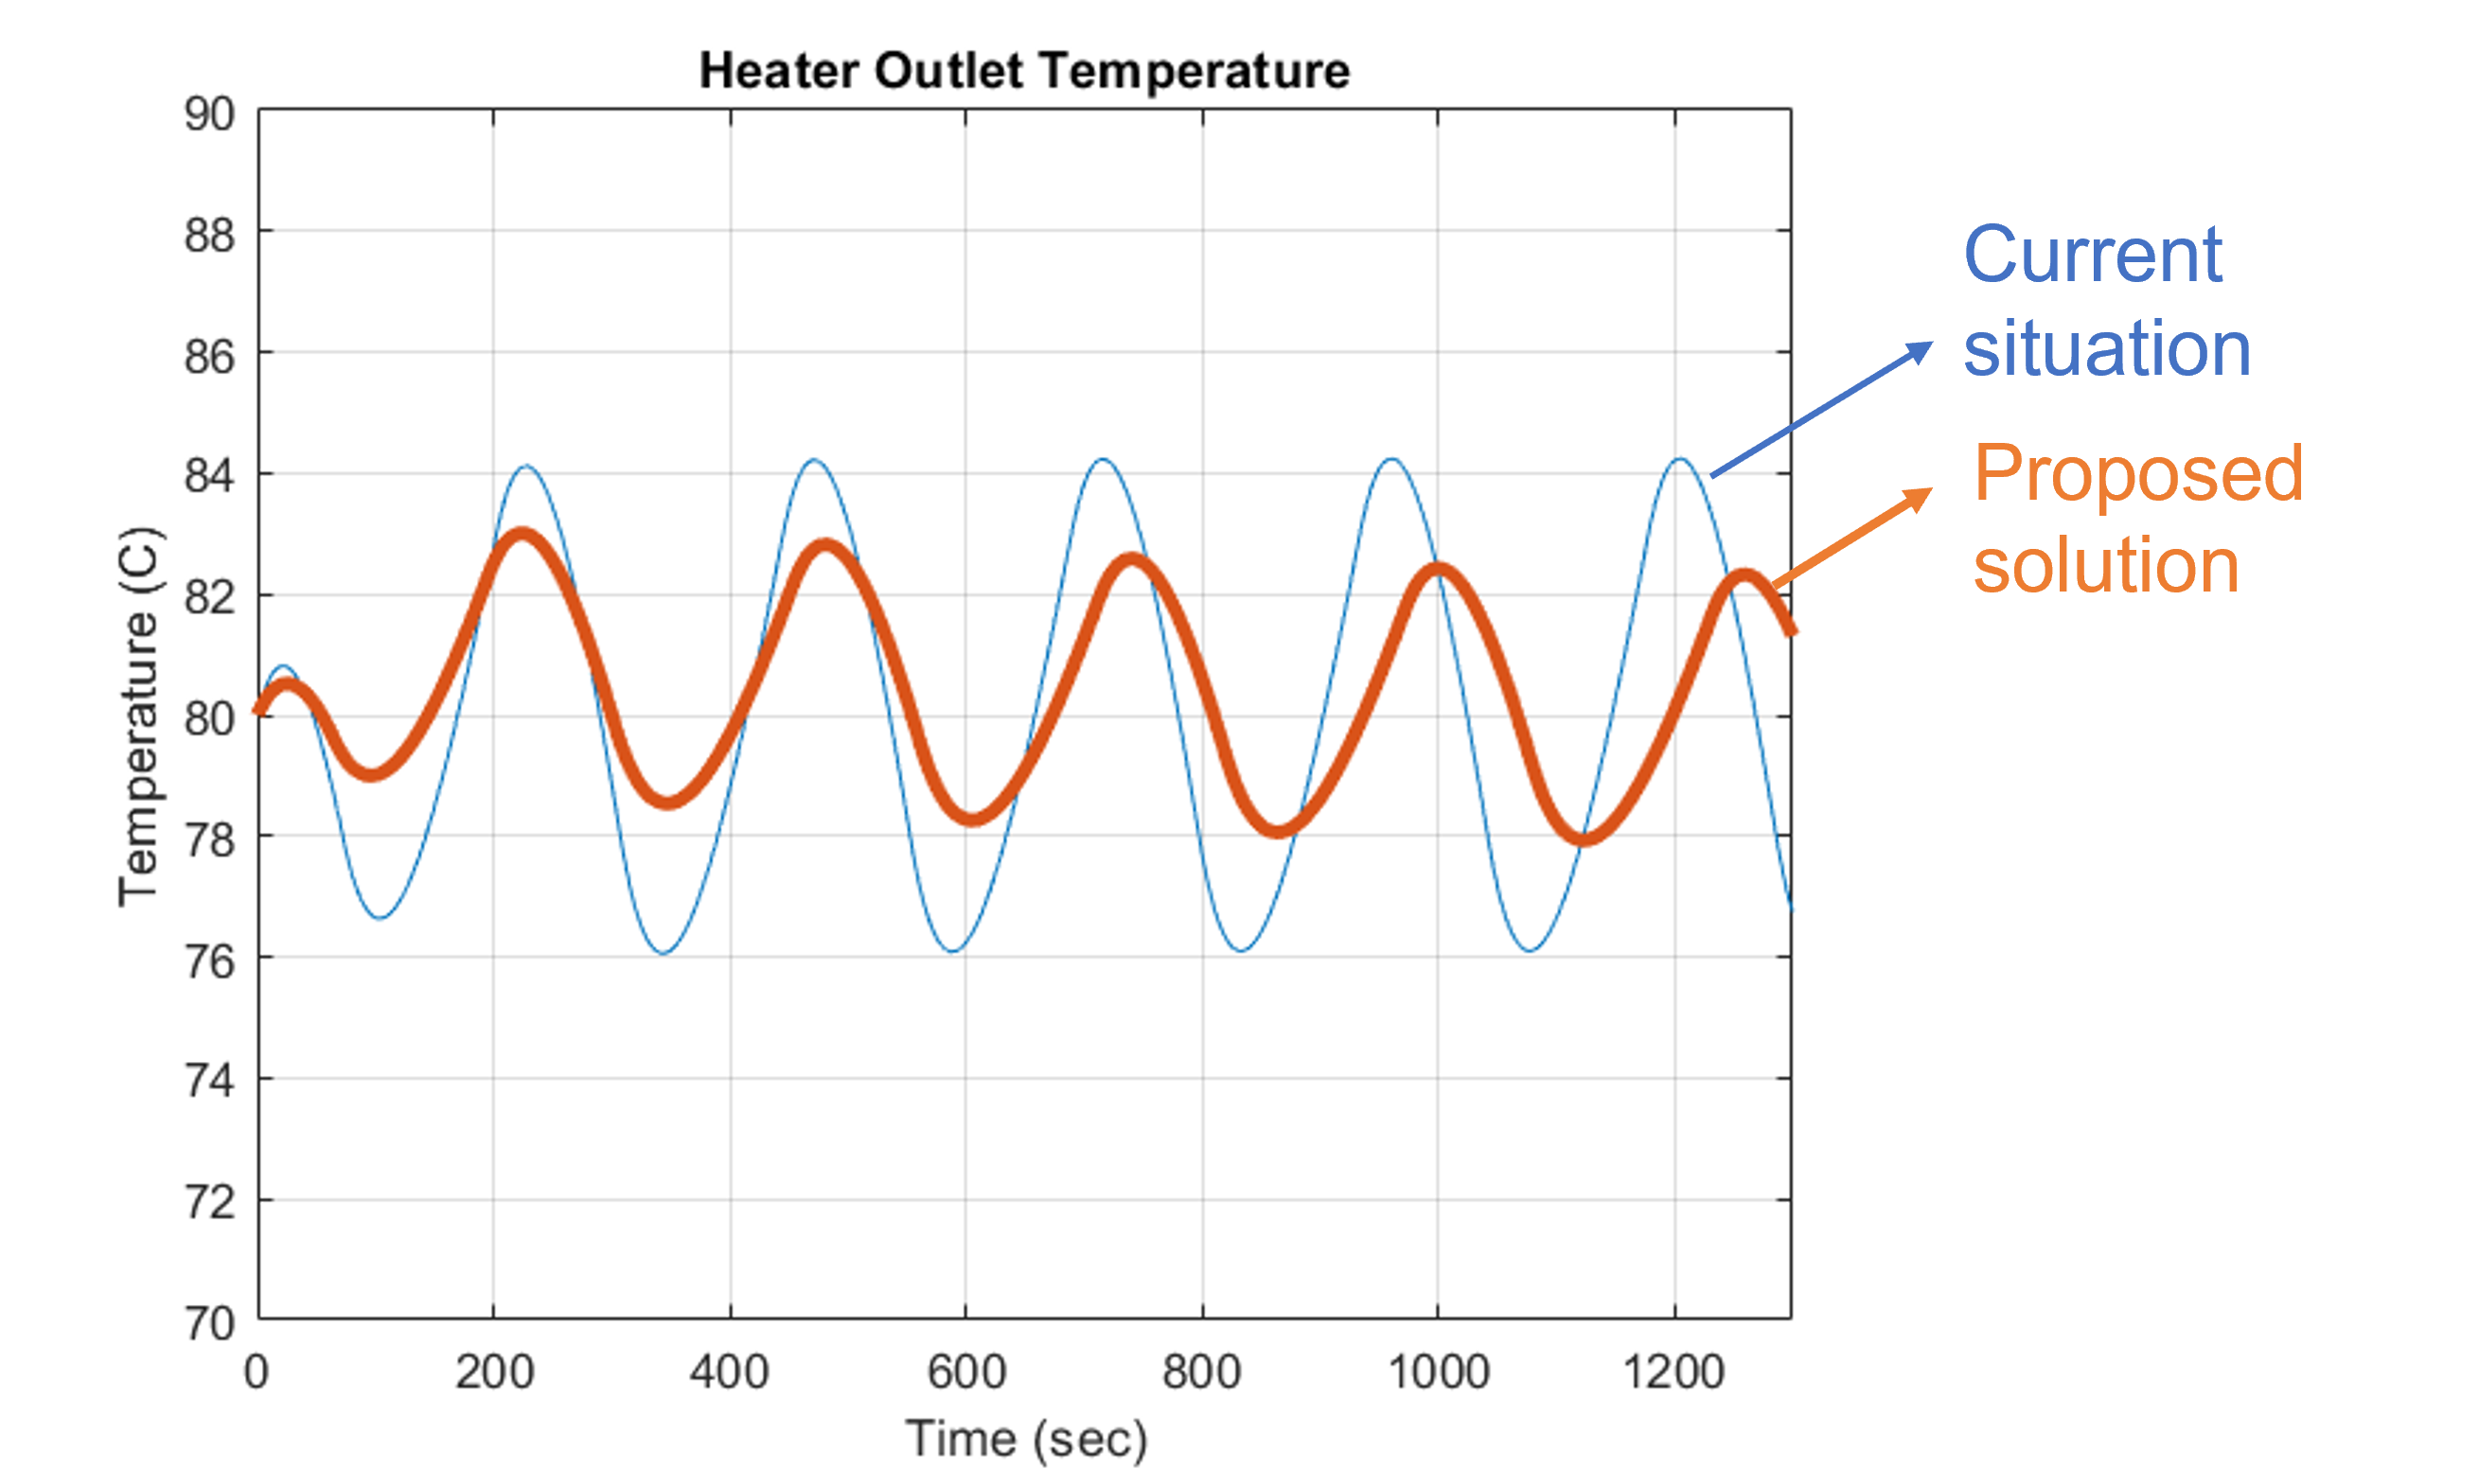
\includegraphics[width=12cm]{images/result.png}
    \caption{Comparison of temperature oscillation results with the solution.}
    \label{fig:result}
\end{figure}

As seen in Figure \ref{fig:result}, several things are changed in the system's time response. Firstly, the oscillation amplitude is decreased as expected. Furthermore, the oscillation period is increased, which has no effect on the cycle, either positive or negative. Thus, results are satisfactory in the sense of decreasing the oscillation magnitude.

\par
On the other hand, there are several things to be noted. When the bypass line is used, the set temperature needs to be set to a higher temperature. Also, the oil flowing in the cycle will be at higher temperatures to compensate for the temperature decrease in the evaporator inlet due to mixing with cooler oil. Higher temperatures overall can lead to more heat loss and, eventually, more power consumption. Additionally, higher temperatures in the components can increase material wearing. Lastly, the construction of this bypass system requires some amount of funding which should be taken into account as well.

\par
The system is tested at its limits to find out how much reduction can be maintained by specified bypass percentages and set temperatures. Two different tests are carried out by setting bypass rates of 50\% and 75\%. Results are provided in Tables \ref{tab:50} and \ref{tab:75}:

\begin{table}[h]
    \centering
    \begin{tabular}{|c c|}
        \hline
        Set temperature ($^\circ$C):   &  93 \\
        Bypass rate (\%):   &  50 \\
        Oscillation amplitude before ($^\circ$C):   &  7.0783 \\
        Oscillation amplitude after ($^\circ$C):   &  4.9918 \\
        Oscillation decrease percentage (\%):   &  30 \\
        \hline
    \end{tabular}
    \caption{Limits of the system when bypass rate is 50\%.}
    \label{tab:50}
\end{table}

\begin{table}[h]
    \centering
    \begin{tabular}{|c c|}
        \hline
        Set temperature ($^\circ$C):   &  120 \\
        Bypass rate (\%):   &  75 \\
        Oscillation amplitude before ($^\circ$C):   &  7.0783 \\
        Oscillation amplitude after ($^\circ$C):   &  3.0159 \\
        Oscillation decrease percentage (\%):   &  57 \\
        \hline
    \end{tabular}
    \caption{Limits of the system when bypass rate is 75\%.}
    \label{tab:75}
\end{table}

\par
As a result, it is seen that the maximum decrease in oscillations can be achieved by 57\% with the maximum operating temperature for 80 $^\circ$C and 75\% bypass rate. Thus, considering the drawbacks mentioned above, this reduction is seen as not sufficient enough to construct the real system. Still, this model can be used for other investigation purposes in the oil cycle. Furthermore, this modeling process can be a guideline for researchers who want to model a power cycle in Matlab/Simulink.   


    \chapter{Conclusion}

The purpose of this report is to address the issue of oscillation in the temperature of the oil in an ORC (organic rankine cycle) system. This oscillation is caused by the heater in the oil cycle overshooting or undershooting the desired temperature. To solve this problem, a dynamic model was developed using Matlab/Simulink, which incorporates thermodynamic and heat transfer equations to simulate the various components of the oil cycle. This model was then validated by comparing it to experimental data, which showed that the model accurately represents the real system. To address the issue of oscillation, a solution was proposed in which a bypass pipeline is created between the inlet and exit of the oil cycle, allowing for reverse flow. This solution was simulated using the validated model, and the results showed that the oscillations could be significantly reduced by adjusting the flow through the bypass pipeline. However, since the resistor can not endure too high temperatures, there is a limit to the set temperature, which bounds the mass flow rate that can flow through the bypass line. Therefore, the oscillations cannot be reduced a lot when the set temperature is high. To test the proposed solution in a real system, an experimental concept setup was designed using a pump, a check valve, a 3-way valve, and an actuator. However, the actual experiment only utilized a 3-way valve and an actuator to demonstrate that the flow direction of the fluid could be controlled using these two components.

    
    \renewcommand\bibname{References} % Change Bibliography to References
    \bibliographystyle{unsrt}
    \bibliography{references.bib}

    \appendix
    \chapter{Simulink Model}
\label{appa}

\section{Cycle Model}
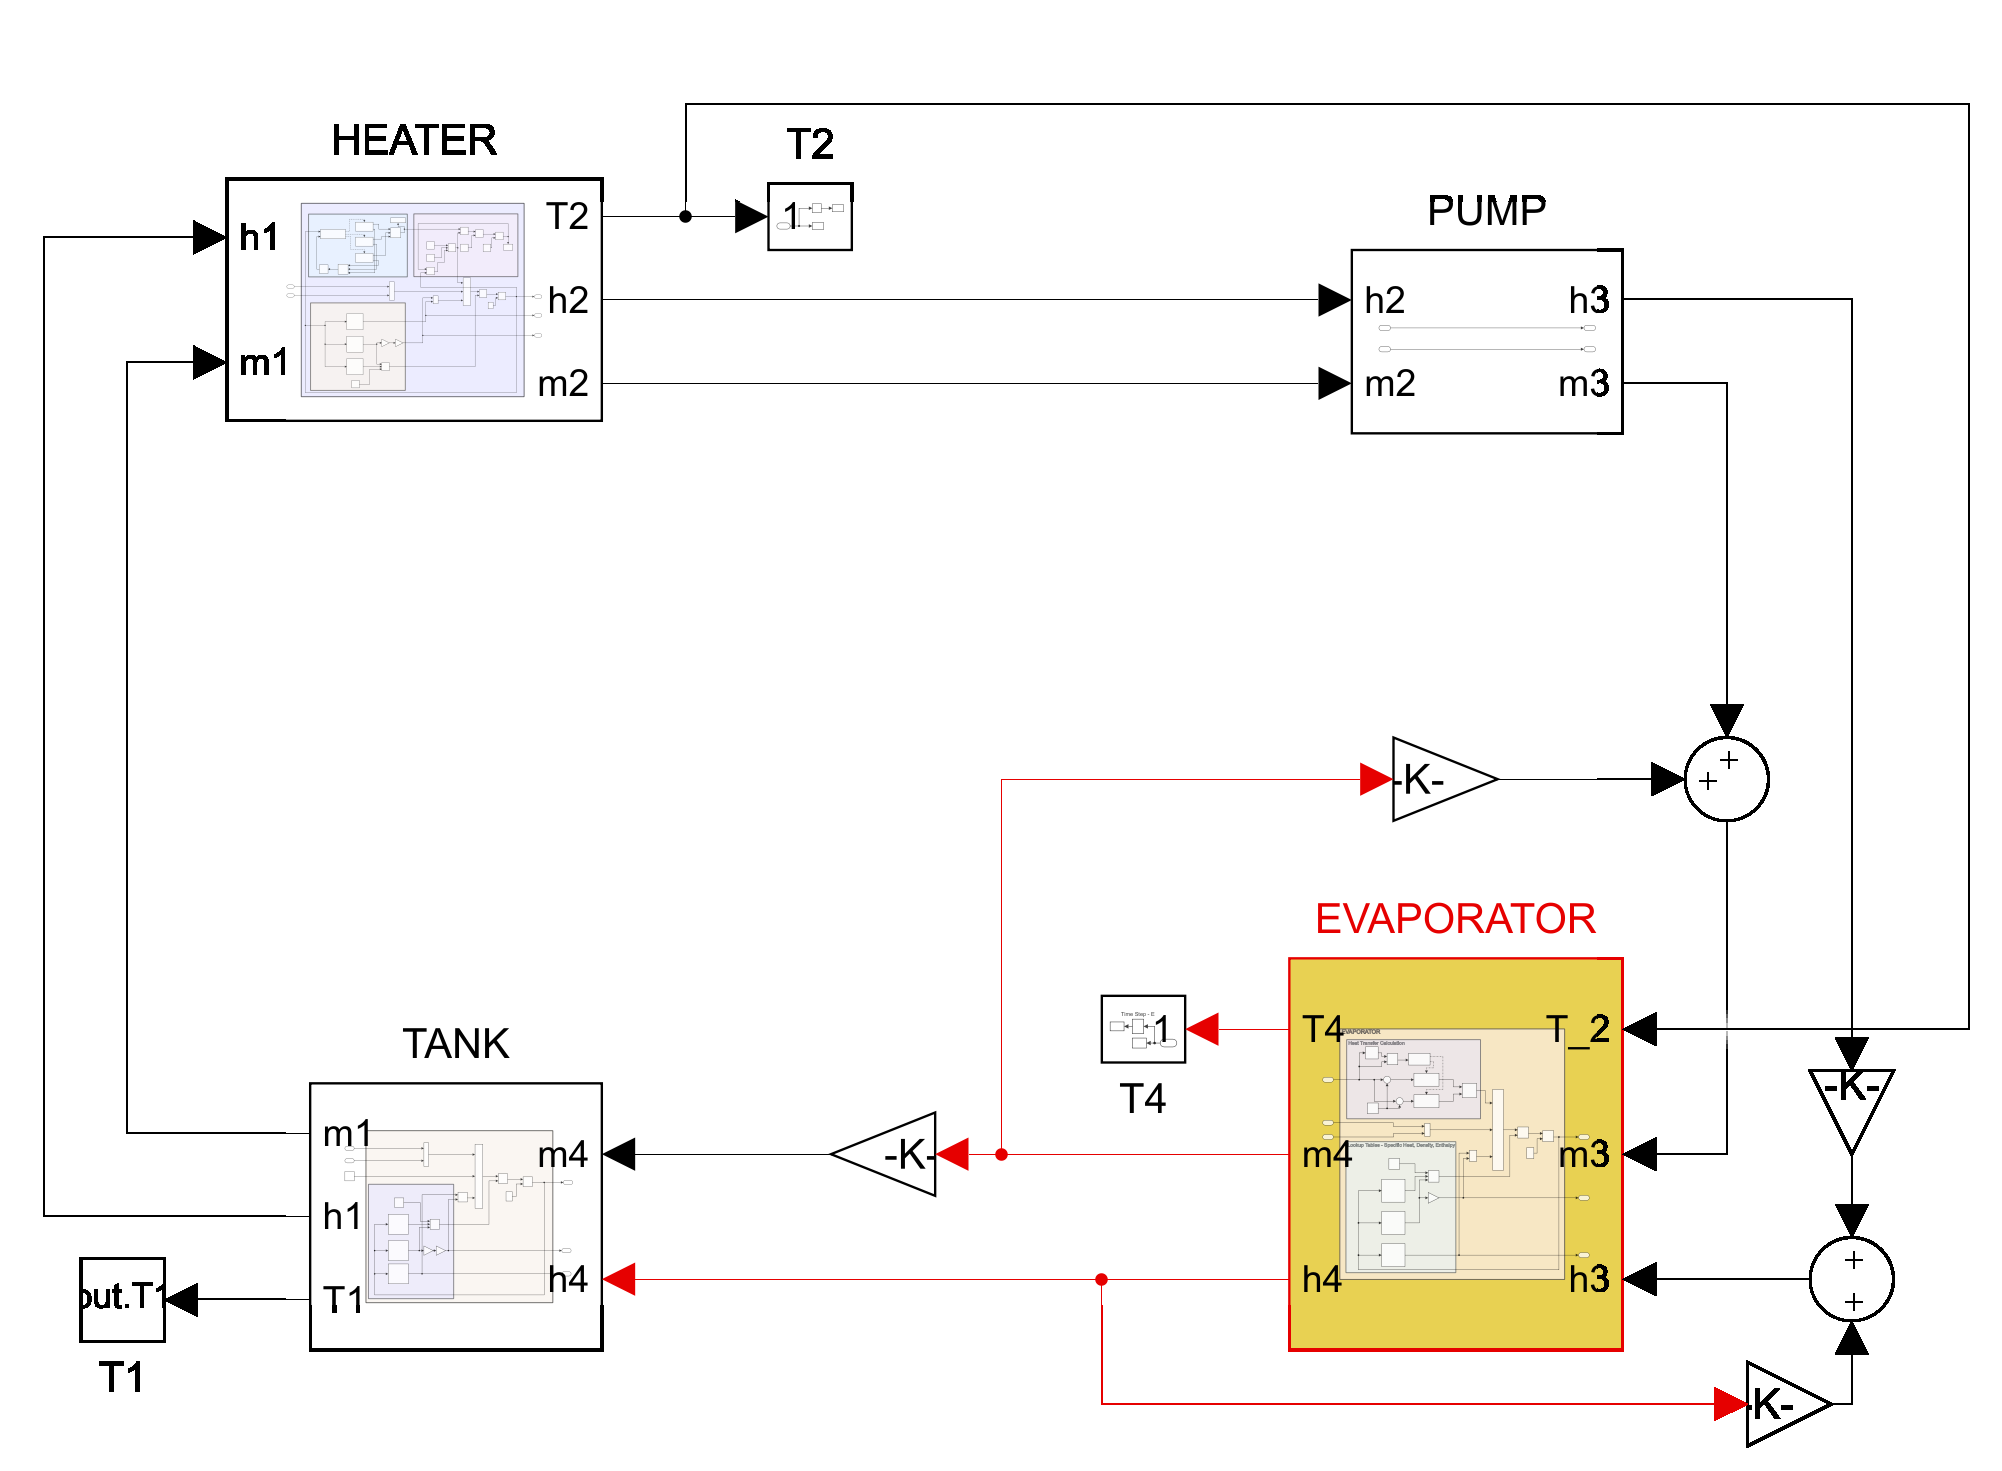
\includegraphics[width=16cm]{images/total-model.png}

\section{Heater Model}
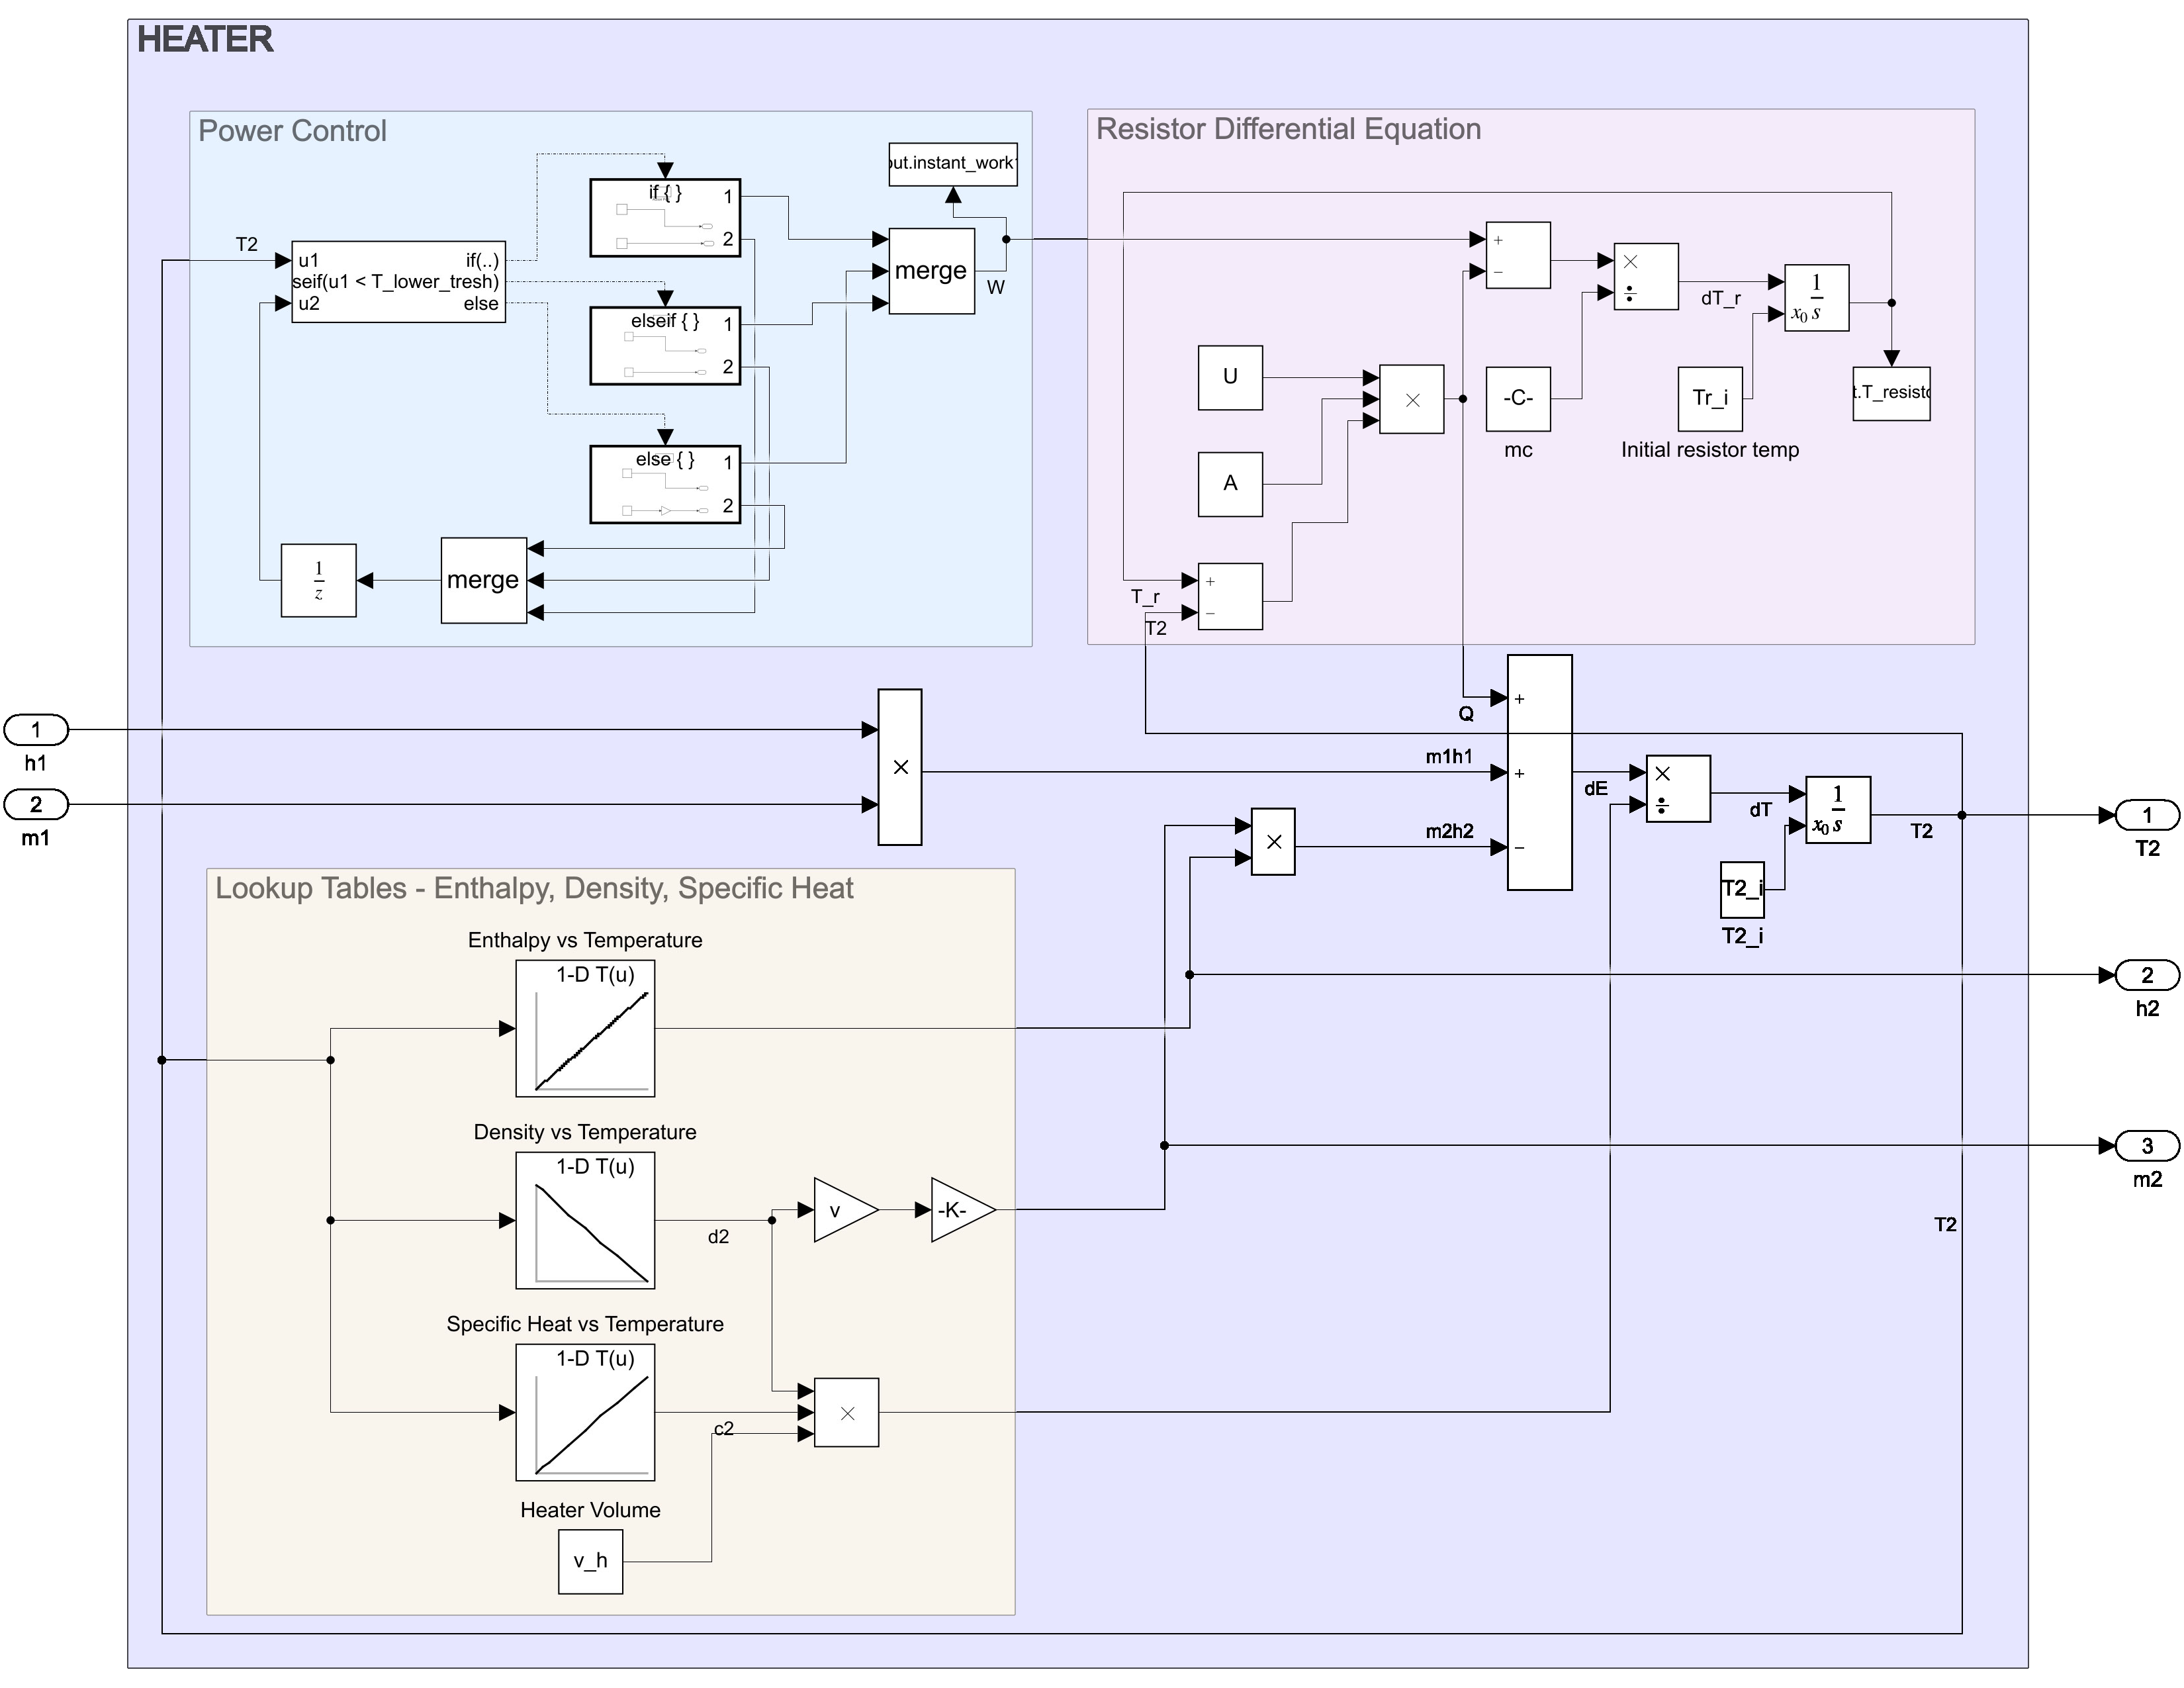
\includegraphics[width=16cm]{images/heater-model.png}

\section{Evaporator Model}
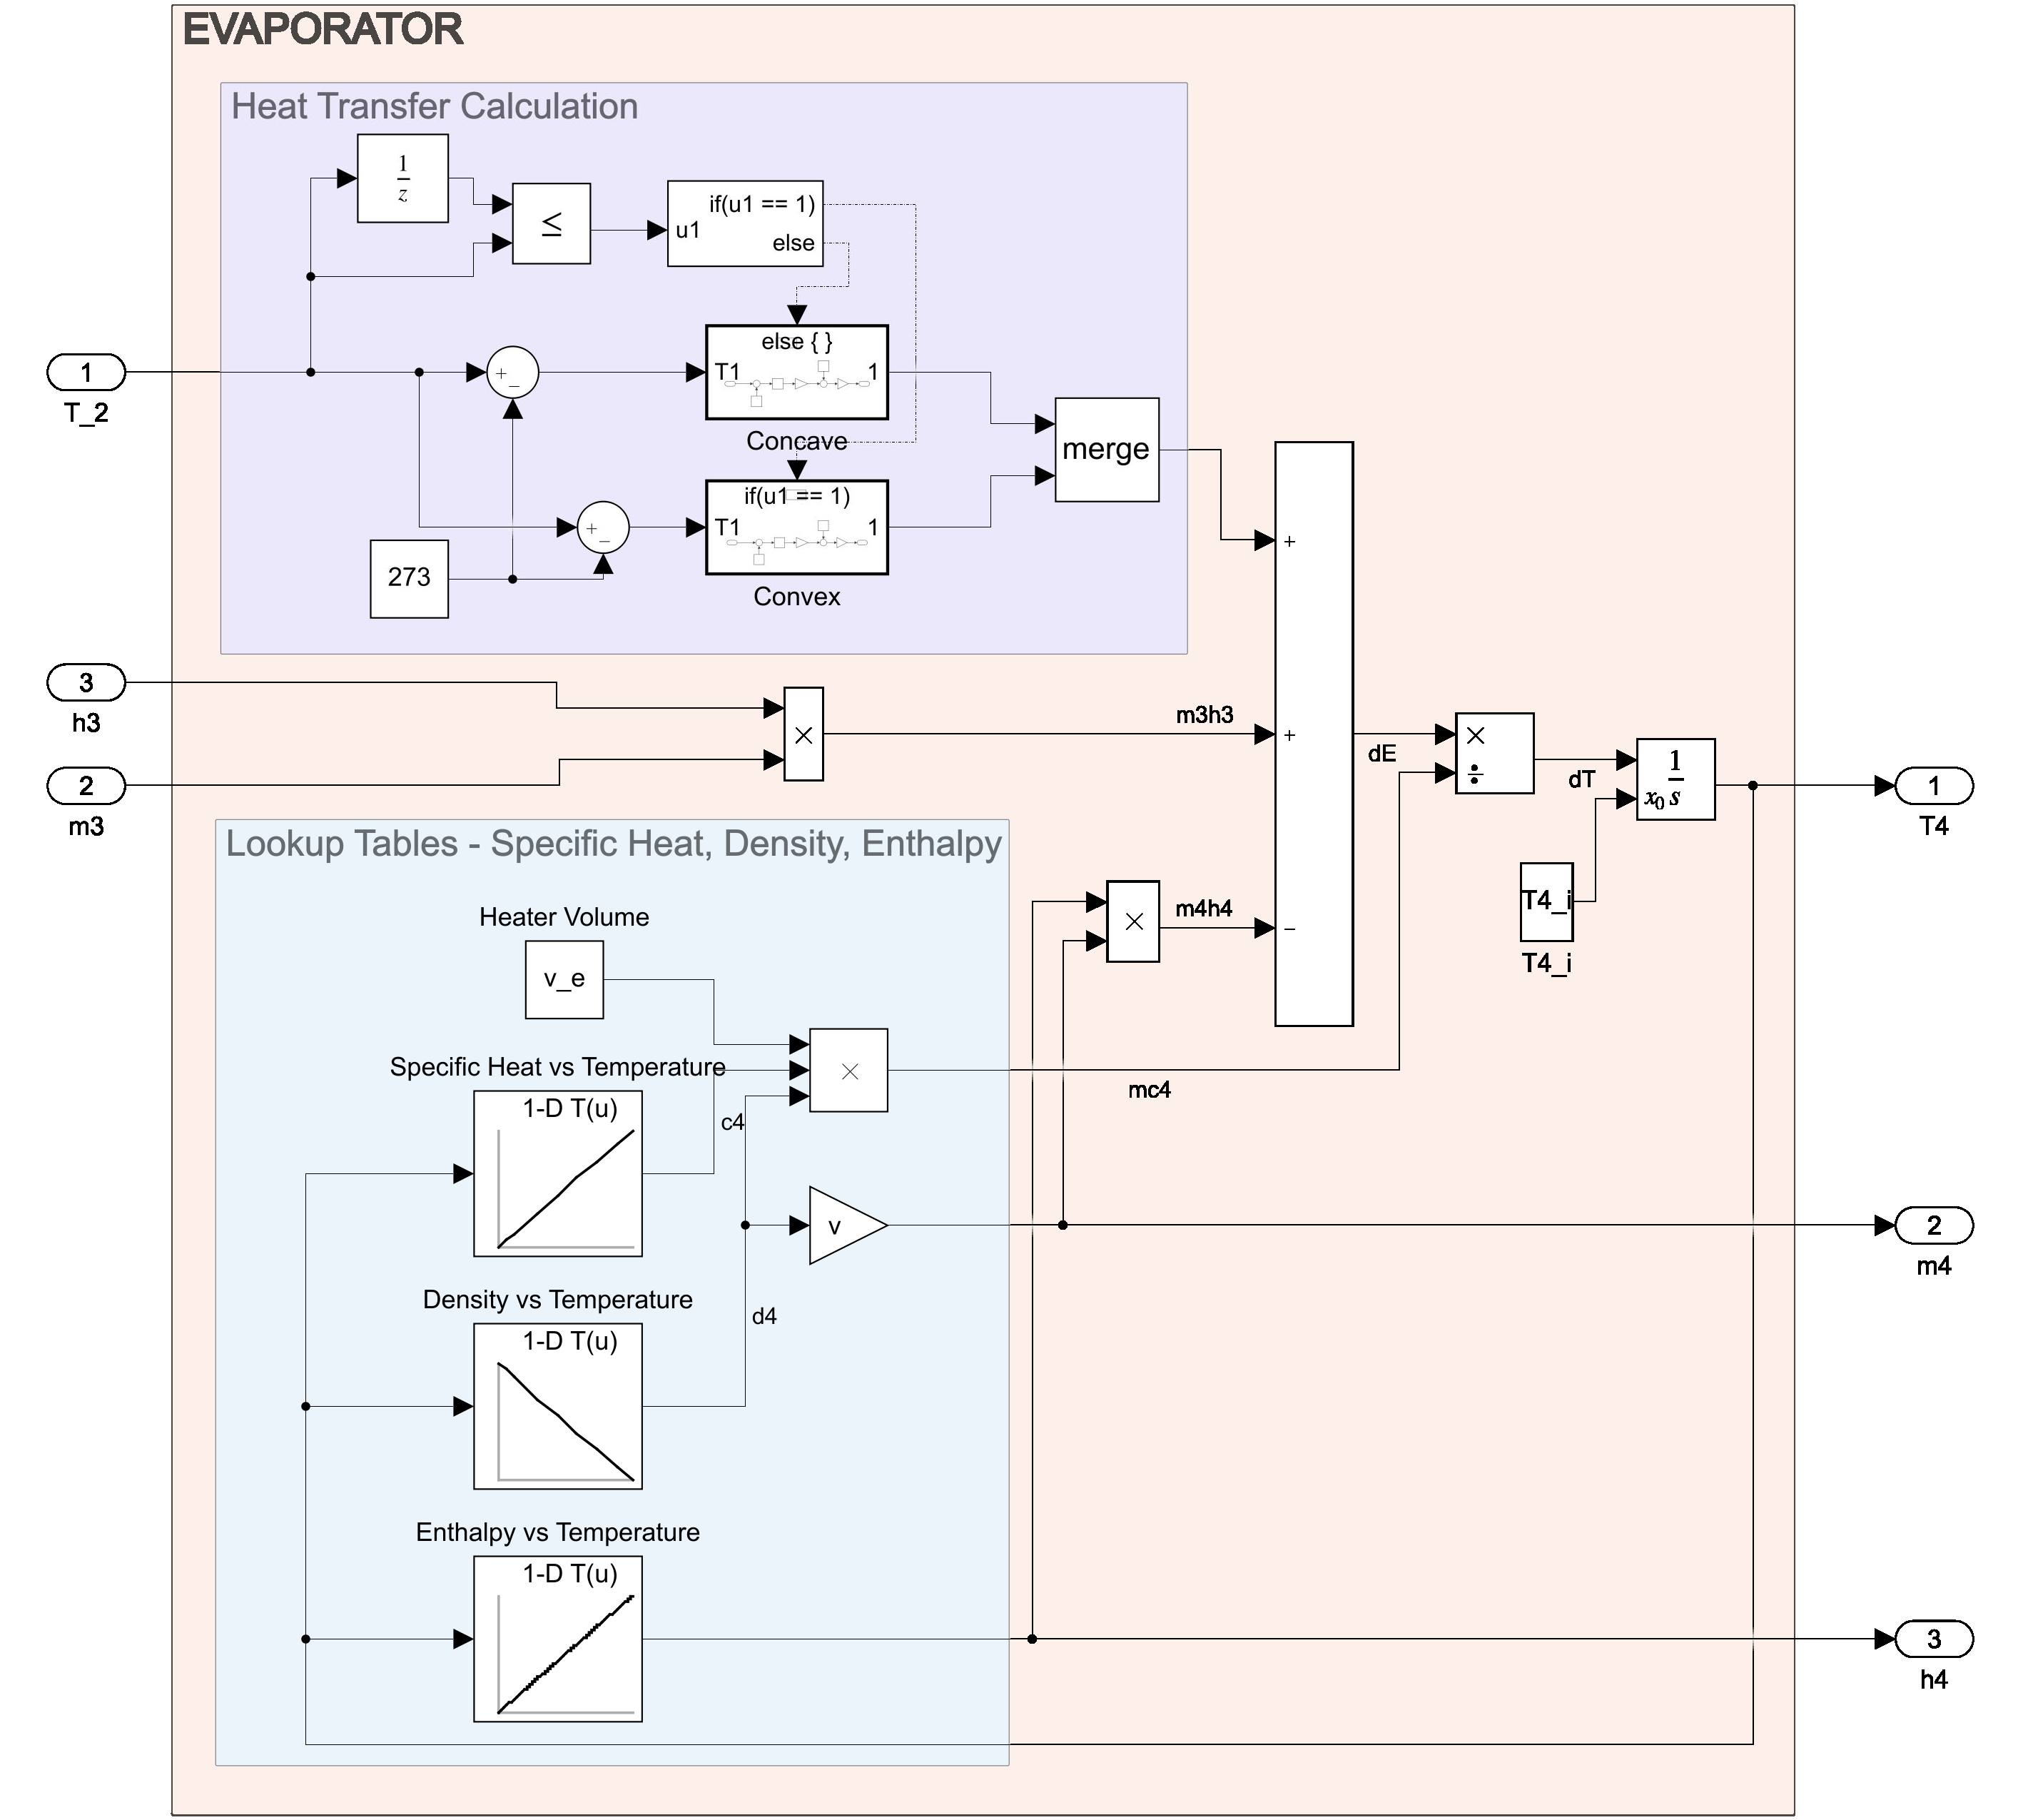
\includegraphics[width=16cm]{images/evaporator-model.png}

\section{Tank Model}
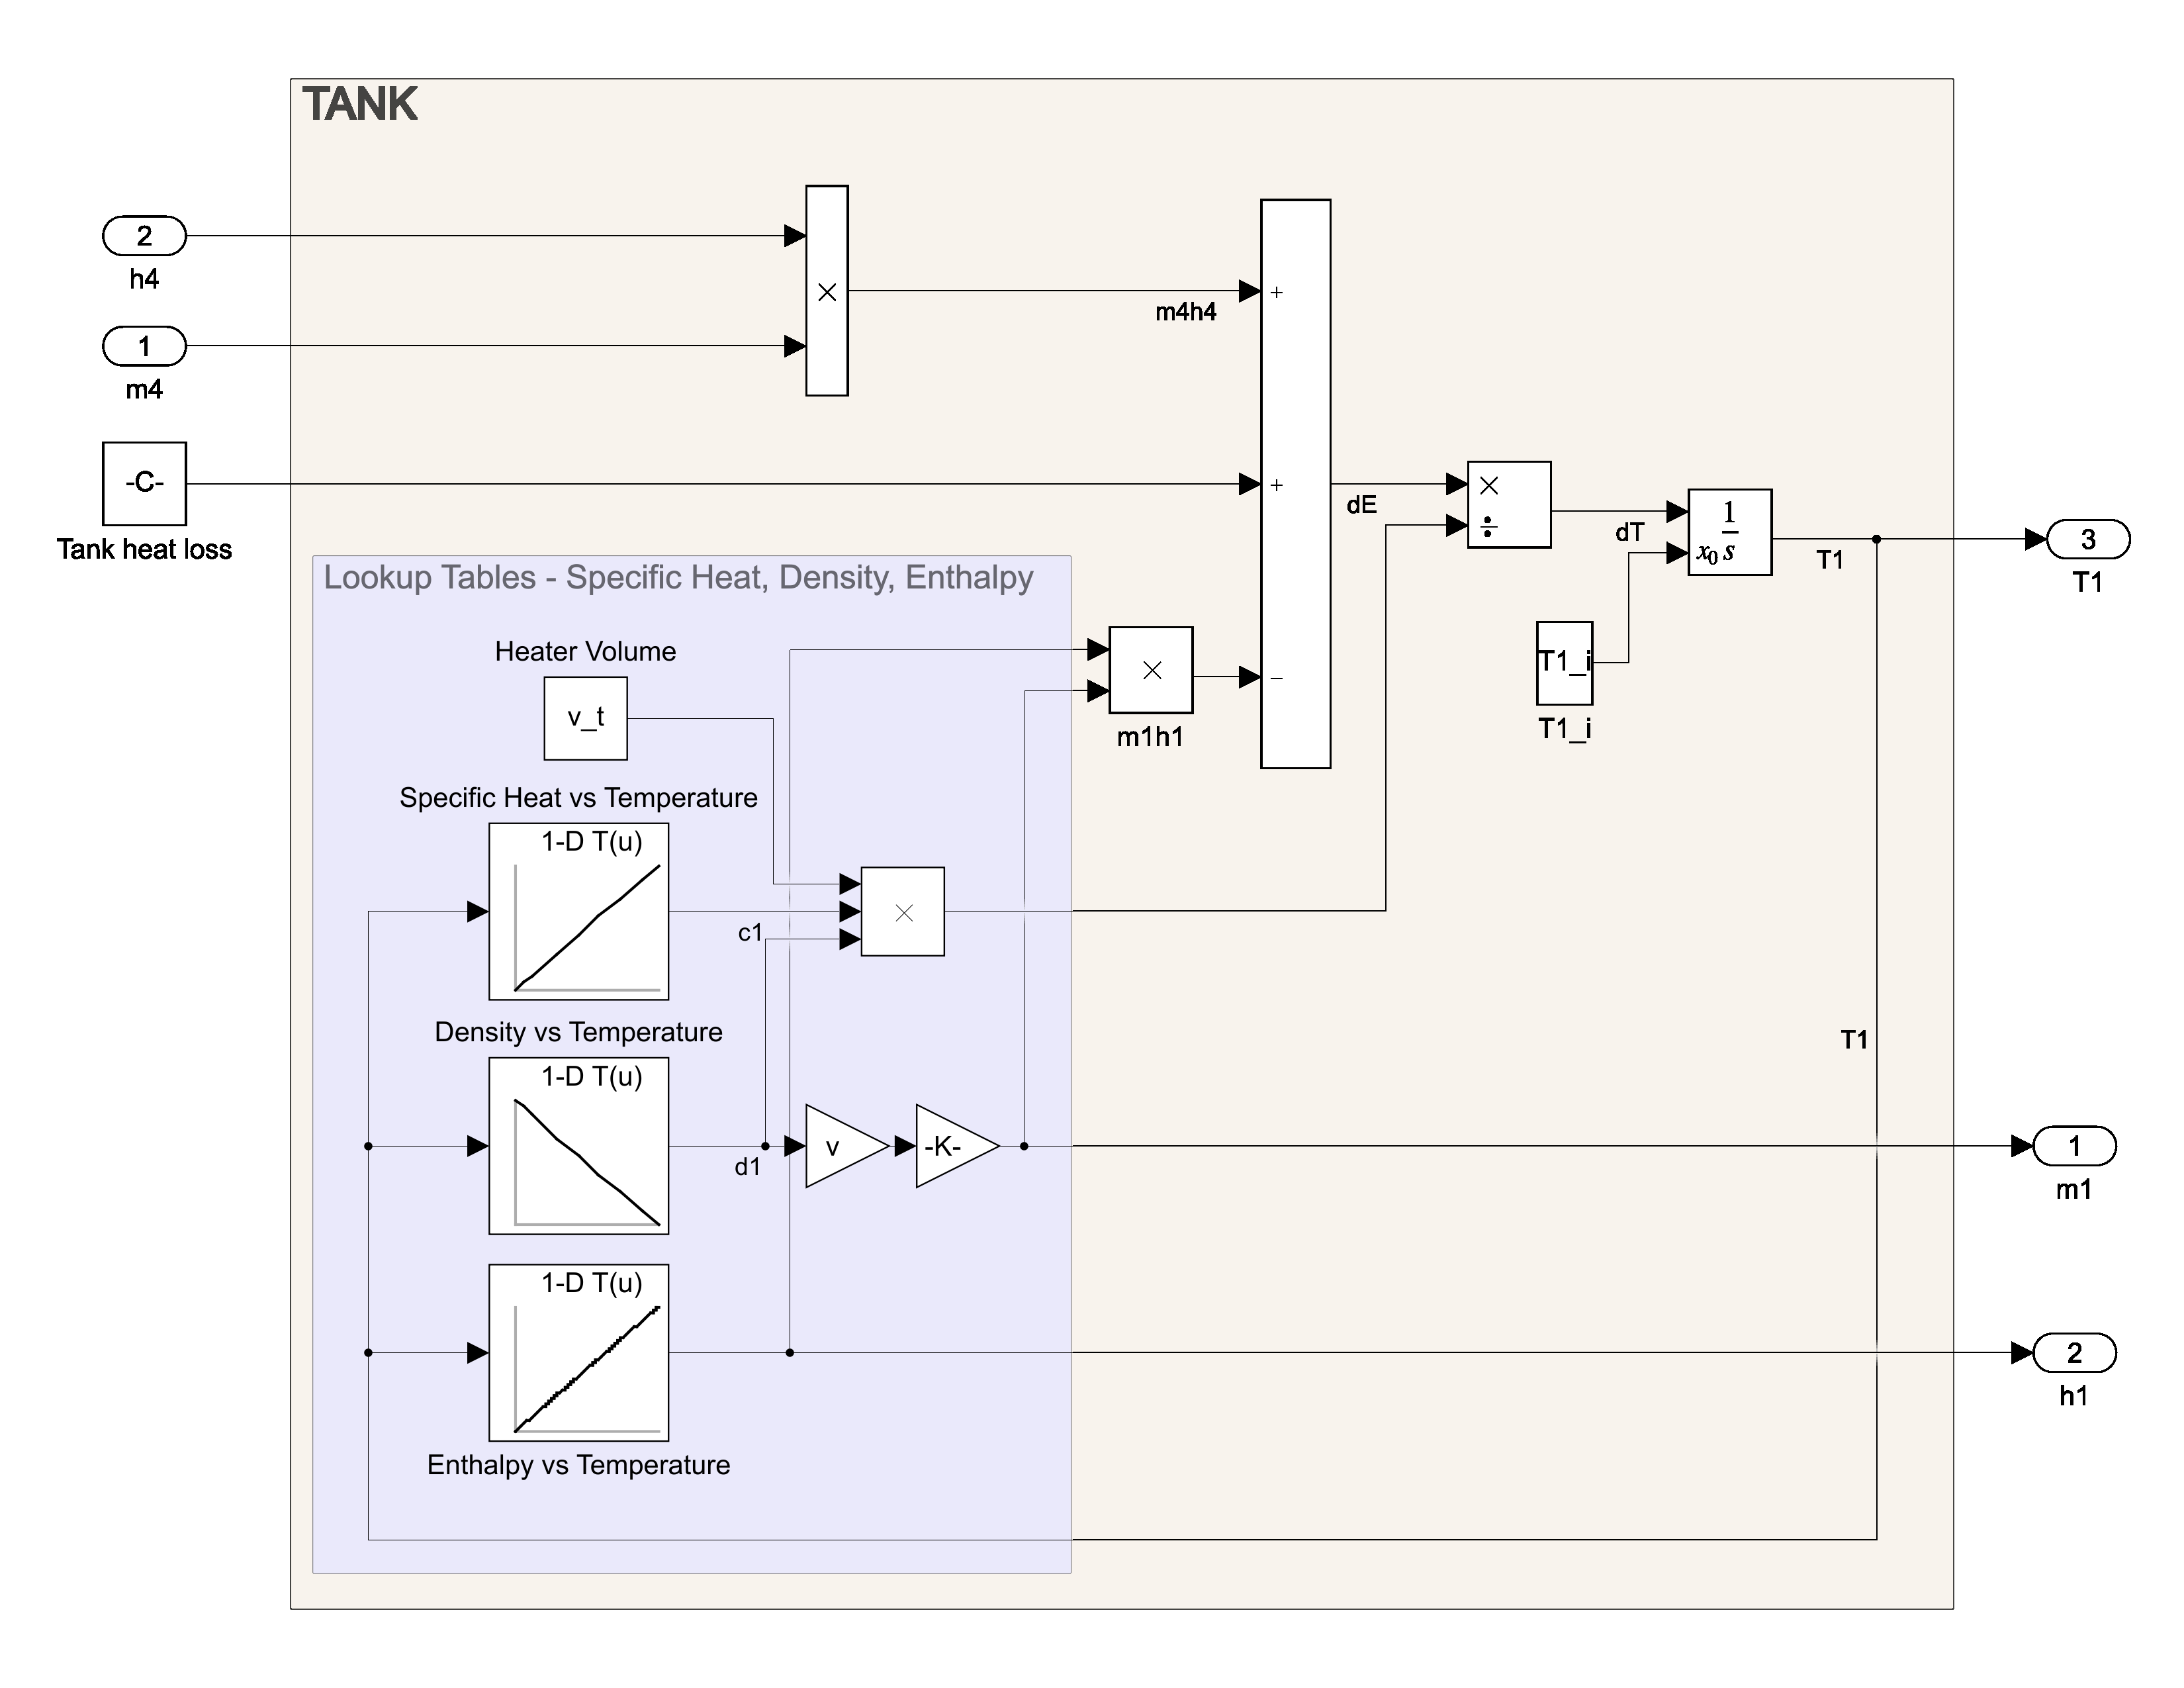
\includegraphics[width=16cm]{images/tank-model.png}

\chapter{Matlab Codes}


\section{Main Live Script}
\label{T_7D74494B}

\begin{par}
\begin{flushleft}
\textit{Load expirmental data:}
\end{flushleft}
\end{par}

\begin{matlabcode}
load("exp_data.mat")
\end{matlabcode}

\label{H_B0204B1A}
\matlabheadingthree{Select Test:}

\begin{par}
\hfill \break
\end{par}

\begin{matlabcode}
test = 1; % select section of experimental data
switch test
    case 0
        % choose manual set temperature
    case 1
        T_set = 80 + 273; % test1 80 
        lower_boundary = 220; 
        upper_boundary = 2400; 
    case 2
        T_set = 110 + 273; % test2 110
        lower_boundary = 2731;
        upper_boundary = 5000;
    case 3
        T_set = 80 + 273; % text3 80 
        lower_boundary = 6300;
        upper_boundary = 8277;
    case 4
        T_set = 100 + 273; % test4 100 
        lower_boundary = 8361;
        upper_boundary = 11096;
    case 5
        T_set = 80 + 273; % test5 80 
        lower_boundary = 12257;
        upper_boundary = 14674;
    case 6
        T_set = 90 + 273; % test6 90
        lower_boundary = 15400;
        upper_boundary = 17700;
    case 7
        T_set = 80 + 273; % test7 80
        lower_boundary = 18188;
        upper_boundary = 20743;
end
\end{matlabcode}

\label{H_68411354}
\matlabheading{\underline{Parameters:}}

\begin{matlabcode}
v = 0.001278; % volumetric flow rate (constant)
\end{matlabcode}

\label{H_B9840D72}
\matlabheadingtwo{\underline{\textbf{Set Bypass Rate:}}}

\begin{matlabcode}
Rate = 0; % bypass rate percentage
bypassRate = Rate/100;     
\end{matlabcode}

\begin{par}
\begin{flushleft}
\textit{If bypass:}
\end{flushleft}
\end{par}

\begin{matlabcode}
%add = (T_set-340)/(1-bypassRate)*bypassRate;
%T_set = T_set + add;
\end{matlabcode}

\label{H_E80BE0AF}
\matlabheadingtwo{\underline{Set Temperature:}}

\begin{matlabcode}
if test == 0
    
    T_set =    80 + 273; % set temperature (K)
    
end
\end{matlabcode}

\begin{par}
\begin{flushleft}
\textit{Set thresholds:}
\end{flushleft}
\end{par}

\begin{matlabcode}
T_upper_tresh = T_set + 3;
T_lower_tresh = T_set - 3.5;
\end{matlabcode}

\label{H_A733F37E}
\matlabheadingtwo{\underline{\textbf{Set Resistor Parameters:}}}

\begin{matlabcode}
W =      100; % input work 
m_r =    20; % resistor's mass
c_r =    0.4; % resistor's c (kJ/kgK)
U =      0.27; % overall heat transfer coefficient (kW/m2K)
A =      1; % area of the resistor (m2)
Tr_i =   T_set; % initial resistor temperature (K)
\end{matlabcode}

\label{H_E6FB3D28}
\matlabheadingthree{Q\_e fit:}

\begin{par}
\hfill \break
\end{par}

\begin{matlabcode}
% concav
a_cv_int = [-0.1919 -0.2681];
b_cv_int = [-80.2397 -110.964];
c_cv_int = [36.531 19.2292];
a_cv = interp1([353 383], a_cv_int, T_set);
b_cv = interp1([353 383], b_cv_int, T_set);
c_cv = interp1([353 383], c_cv_int, T_set);

% convex
a_cx_int = [0.3102 0.1053];
b_cx_int = [-79.1199 -109.644];
c_cx_int = [24.3597 11.8066];
a_cx = interp1([353 383], a_cx_int, T_set);
b_cx = interp1([353 383], b_cx_int, T_set);
c_cx = interp1([353 383], c_cx_int, T_set);
\end{matlabcode}

\label{H_445E186B}
\matlabheadingthree{Q\_loss fit:}

\begin{par}
\hfill \break
\end{par}

\begin{matlabcode}
Q_tank = -7.4074e-06*(T_set-273-110)^4 - 8; % quadratic fit
\end{matlabcode}

\label{H_628676B0}
\matlabheadingthree{\textbf{Density \& Specific Heat Lookup Tables:}}

\begin{par}
\hfill \break
\end{par}

\begin{matlabcode}
T_lookup = [0 20 40 100 150 200 250 300 340] + 273;
d_lookup = [871 858 845 804 773 741 708 676 651];
c_lookup = [1.962 2.049 2.137 2.4 2.619 2.838 3.058 3.277 3.452];
\end{matlabcode}

\begin{par}
\begin{flushleft}
\textbf{Heater parameters:}
\end{flushleft}
\end{par}

\begin{matlabcode}
v_h =       0.29; % oil's volume in the heater
T2_i =     T_set; % initial oil temperature in the heater
\end{matlabcode}

\begin{par}
\begin{flushleft}
\textbf{Evaporator parameters:}
\end{flushleft}
\end{par}

\begin{matlabcode}
v_e =    0.00384;                % oil's volume in the evaporator
T4_i =   T_set - 13;             % initial oil temperature in evaporator
\end{matlabcode}

\begin{par}
\begin{flushleft}
\textbf{Tank parameters:}
\end{flushleft}
\end{par}

\begin{matlabcode}
v_t =   0.167;                  % oil's volume in the tank + pipes
T1_i =  T_set - 13;             % initial oil temperature in tank
\end{matlabcode}

\label{H_B8536940}
\matlabheading{\underline{Results:}}

\begin{par}
\begin{flushleft}
\textit{Simulation:}
\end{flushleft}
\end{par}

\begin{matlabcode}
out = sim('OilHeaterModel', 2300);
T1 = out.T1.Data - 273;
T2 = out.T2.Data - 273;
T4 = out.T4.Data - 273;

time = out.T1.Time;
\end{matlabcode}

\begin{par}
\begin{flushleft}
\textit{Temperature after bypass at evaporator inlet:}
\end{flushleft}
\end{par}

\begin{matlabcode}
T2_updated = T4*bypassRate + T2*(1-bypassRate);
\end{matlabcode}

\begin{par}
\begin{flushleft}
\textit{Oscillation magnitudes before and after bypass:}
\end{flushleft}
\end{par}

\begin{matlabcode}
O_magnitude_before = max(T2) - min(T2)
O_magnitude_after = max(T2_updated(70150:end)) - min(T2_updated(70150:end))
\end{matlabcode}

\label{H_97B524D0}
\matlabheadingtwo{\textbf{Plot:}}

\begin{matlabcode}
figure
plot(time, T1)
grid on, hold on
title("Tank Outlet Temperature")
xlabel("Time (sec)")
ylabel("Temperature (C)")
ylim([0 100])
xlim([0 1300])

figure
plot(time, T2)
grid on, hold on
title("Heater Outlet Temperature")
xlabel("Time (sec)")
ylabel("Temperature (C)")
ylimits = [T_set-273-10 T_set-273+10];
ylim(ylimits)
xlim([0 1300])

figure
plot(time, T2_updated)
grid on, hold on
title("Evaporator Inlet Temperature")
xlabel("Time (sec)")
ylabel("Temperature (C)")
ylim(ylimits)
xlim([0 1300])

figure
plot(time, T4)
grid on, hold on
title("Evaporator Outlet Temperature")
xlabel("Time (sec)")
ylabel("Temperature (C)")
ylim([40 120])
xlim([0 1300])
\end{matlabcode}

\clearpage

\section{Training \& Validation Script}

\begin{matlabcode}
T2_step = out.T2_step.Data;
T2_step_ein = zeros(2300,1);
j = 1;

for i=1:length(T2_step)
    if T2_step(i) > 0
        T2_step_ein(j) = T2_step(i);
        j = j + 1;
        if j > 2300
            break;
        end
    end
end
T_model_ein = T2_step_ein(1001:end) - 273; 

T4_step = out.T4_step.Data;
T_step_eout = zeros(2300,1);
k = 1;

for i=1:length(T4_step)
    if T4_step(i) > 0
        T_step_eout(k) = T4_step(i);
        k = k + 1;
    end
end
T_model_eout = T_step_eout(1001:end) - 273;  

T_exp_ein = T_ein(lower_boundary:upper_boundary); 

initial = T_model_ein(1); 

slop = T_model_ein(2)-T_model_ein(1) > 0;

min_error = 10;
starting_index = 1;
for i=1:500
    error = abs(initial - T_exp_ein(i));
    exp_slop = (T_exp_ein(i+1) - T_exp_ein(i)) > 0;
    if error < min_error && exp_slop == slop
        starting_index = i;
        min_error = error;
    end
end
T_exp_ein = T_exp_ein(starting_index:starting_index+1299);

mse = (T_model_ein - T_exp_ein)'*(T_model_ein - T_exp_ein)/1300

fig = figure;
plot(T_model_ein)
hold on, grid on
plot(T_exp_ein)
xlim([0 1300])
ylim(ylimits)
title("Evaporator Inlet Temperature", sprintf("TEST-%g: %g C", test, T_set-273))
xlabel("Time (sec)")
ylabel("Temperature (C)")
legend("Model", "Experiment")

text = 'C:\Users\ASUS\Desktop\Test-Results\TEST-' + sprintf("%g.png", test);
saveas(fig, text)
\end{matlabcode}



\end{document}
